\documentclass{article}

\usepackage[utf8]{inputenc}
\usepackage[english]{babel}

\usepackage{amssymb}
\usepackage{amsmath}
\usepackage{mathtools} % \coloneqq, which is :=, \lfloor, \rfloor
\usepackage{verbatim}
\usepackage{physics}
\usepackage{geometry}
\usepackage{float}
\usepackage{hyperref}
\usepackage{graphicx}
\usepackage{slashed} % Feynman slash notation
\usepackage{listings} % for code listings
\usepackage{svg} % svg images
\usepackage{pythontex} % python code within the document
\usepackage{enumitem} % customising enumeration ex: 1), 2), 3), ...
\usepackage{cancel} % strikethrough equations
\usepackage[group-separator={,}]{siunitx} % thousand separator in large numbers
\usepackage[nottoc,numbib]{tocbibind} % references in toc
\usepackage[ruled,vlined,linesnumbered]{algorithm2e} % pseudocode listings

% definition of all the colors
\usepackage{array}
\usepackage{xcolor,colortbl}
%
% genertated by ./compile.py
%

\definecolor{codegreen}{RGB}{0, 153, 0}
\definecolor{codegray}{RGB}{127, 127, 127}
\definecolor{codeblue}{RGB}{102, 214, 237}
\definecolor{codekeyword}{RGB}{249, 36, 114}
\definecolor{codecomment}{RGB}{127, 127, 127}
\definecolor{backcolor}{RGB}{242, 242, 235}
\definecolor{linkcolor}{RGB}{102, 0, 0}
\definecolor{corange}{RGB}{255, 70, 0}
\definecolor{cyellow}{RGB}{209, 153, 0}
\definecolor{cblue}{RGB}{64, 128, 255}
\definecolor{cbrown}{RGB}{153, 102, 51}
\definecolor{cpink}{RGB}{255, 0, 255}
\definecolor{cred}{RGB}{255, 64, 0}
\definecolor{cgreen}{RGB}{0, 191, 0}
\definecolor{clightblue}{RGB}{191, 217, 255}
\definecolor{cturquois}{RGB}{0, 255, 255}
\definecolor{cpurple}{RGB}{128, 0, 255}
\definecolor{clightgreen}{RGB}{175, 255, 175}
\definecolor{clightpink}{RGB}{255, 175, 255}
\definecolor{cdarkblue}{RGB}{0, 0, 255}
\definecolor{cdarkred}{RGB}{255, 0, 0}
\definecolor{cdarkgreen}{RGB}{0, 255, 0}


% setup for the \num, siunitx package
%\sisetup{round-mode = figures}

% appearance of the hyperlinks in the text
\hypersetup{
  linkcolor  = linkcolor,
  citecolor  = linkcolor,
  urlcolor   = linkcolor,
  colorlinks = true,
}

%Code listing style named "codestyle"
\lstdefinestyle{codestyle}{
    backgroundcolor=\color{backcolor},
    commentstyle=\color{codecomment},
    keywordstyle=\color{codekeyword},
    numberstyle=\tiny\color{codegray},
    stringstyle=\color{codestring},
    basicstyle=\ttfamily\footnotesize,
    breakatwhitespace=false,
    breaklines=true,
    captionpos=b,
    keepspaces=true,
    numbers=left,
    numbersep=5pt,
    showspaces=false,
    showstringspaces=false,
    showtabs=false,
    tabsize=2
}

\lstset{style=codestyle}

\newcommand{\eqname}[1]{\tag*{#1}} % Tag equation with name
% label only one equation on align*, see https://tex.stackexchange.com/a/42728
\newcommand\numberthis{\addtocounter{equation}{1}\tag{\theequation}}

\usepackage{tikz}
\usetikzlibrary{tikzmark} % arrow pointing to character in equation https://tex.stackexchange.com/questions/191217/arrow-pointing-to-subscript-in-equation
\usepackage{standalone} % to include tikzpictures using \includestandalone

%\usepackage[bottom]{footmisc} % put footnote at the bottom of the page https://tex.stackexchange.com/questions/9425/how-to-fix-footnote-position-at-the-bottom-of-the-page

%\interfootnotelinepenalty=10000 % force the footnote to stay on only one page

\usepackage[
    type={CC},
    modifier={by-sa},
    version={4.0}
]{doclicense}

\usepackage{amsthm}
\theoremstyle{plain} % boldface title, italicized body. 
\newtheorem{theorem}{Theorem}[section]
\newtheorem{corollary}{Corollary}[theorem]
\newtheorem{lemma}[theorem]{Lemma}
\newtheorem{prop}[theorem]{Proposition}
%\theoremstyle{definition} % boldface title, roman body.  
\newtheorem{definition}{Definition}[section]
\newtheorem{example}{Example}[section]
\theoremstyle{remark} % italicized title, roman body. 
\newtheorem*{remark}{Remark} % * creates a theorem environment that is not numbered 
\newtheorem{proposal}{Proposal}[section]

\allowdisplaybreaks % page breaks in equations
\graphicspath{{./img/}{./plots/}}

\geometry{
  a4paper,
  left=29mm,
  right=29mm,
  top=20mm,
}

% defines the \code{} command
\def\code#1{\texttt{#1}}

% defines the \def{} command
\def\df#1{\textbf{\textit{#1}}}

\title{Master Thesis \\ Performance Modelling and Analysis of the openQxD Lattice QCD Application}
\author{Roman Gruber}
\date{ETH Zürich, TODO:date, TODO: supervior(s)}

\numberwithin{equation}{section}

\usepackage[acronym,toc]{glossaries} % toc: glossary and acronyms to appear in the table of contents
\makeglossaries
\loadglsentries{include/glossary} % include glossary.tex
\loadglsentries{include/acronyms} % include acronyms.tex

\begin{document}

\maketitle

\begin{abstract}
TODO
\end{abstract}

\doclicenseThis

\noindent\textcolor{gray}{\hrulefill}

\tableofcontents

\noindent\textcolor{gray}{\hrulefill}

\section{Introduction}

TODO

In \acrshort{QCD} blabla. \textcolor{corange}{orange}, \textcolor{cyellow}{yellow}, \textcolor{cblue}{blue}, \textcolor{cbrown}{brown}, \textcolor{cpink}{pink}, \textcolor{cred}{red}, \textcolor{cgreen}{green}, \textcolor{cpurple}{purple}, \textcolor{cturquois}{turquois}, \textcolor{clightblue}{lightblue}, \textcolor{clightgreen}{lightgreen}, \textcolor{clightpink}{lightpink},  \textcolor{cdarkblue}{darkblue}, \colorbox{clightblue}{lightblue}, \colorbox{clightpink}{lightpink}, \colorbox{clightgreen}{lightgreen}, \textcolor{linkcolor}{linkcolor}

\begin{pycode}
from sympy import *
x=symbols('x')
result = latex(integrate("(1+x)**(1/2)",x))
\end{pycode}
 
The result of integrating $\int \sqrt{ 1+x } \, dx$ is given by $\py{result}$

\begin{pycode}
print("Python says ``Hello!''")
\end{pycode}

\section{Conventions}

\section{QCD}

TODO:
non-abelian, hadronic physics, importance, renormalization problems, running coupling, pert theory in high enery phsyics, not in low energy regime

\section{lattice QCD}

TODO: as a renormalization scheme, observables, ...
boundary conditions, specially SF type, 

\section{Performance Models}

TODO: why are they important? semi-analytical, analytical vs. empritical models

\section{Software: openQxD}

the software package openQxD: description
  * importance of CG in openQxD and what it does / how it's used in the software / why 90\% computation time

\section{Conjugate Gradient algorithm}

In many scientific computations large systems of linear equations need to be solved. Usually these systems are huge and the matrices and vectors are distributed among many \glspl{rank}. The method to solve such systems should therefore be iteratively. The problem can be formulated mathematically in the following way. Let $n \in \mathbb{N}$ and let $A$ be a $n \times n$-matrix with components in $\mathbb{C}$, Hermitian, positive definite and \glslink{sparse matrix}{sparse}

\begin{align*}
    A^{\dagger} &= A, &\text{(\df{Hermitian})} \\
    \forall \vec{x} \in \mathbb{C}^n \setminus \{0\} \quad \colon \quad \vec{x}^{\dagger} A \vec{x} &> 0, &\text{(\df{positive definite})}
\end{align*}

as well as $\vec{b} \in \mathbb{C}^n$ be given, then the \df{system of linear equations} can be described as

\begin{align}
    A \vec{x} = \vec{b}. \label{eq:Axb}
\end{align}

We are interested in the \df{solution} vector $\vec{x}$, that is the one that satisfies the above equation, $n$ is called the \df{problem size}. First let us define a function that will be helpfull in the next sections.

\begin{definition}[Quadratic form]

The \df{quadratic form} depends on the problem matrix $A$ as well as on the \df{source} vector $\vec{b}$ and is defined as

\begin{align*}
    f(\vec{x}) = \frac{1}{2} \vec{x}^{\dagger} A \vec{x} - \vec{b}^{\dagger} \vec{x} + c,
\end{align*}

where $c \in \mathbb{C}$. When taking the derivative of this function with repect to $\vec{x}$, we find that

\begin{align*}
    f'(\vec{x}) = A \vec{x} - \vec{b}.
\end{align*}

Therefore finding the extrema of $f(\vec{x})$ is equivalent to solving the linear system of equations \eqref{eq:Axb}. The question whether the solution $\vec{x}$ is unique remains.

\end{definition}

\begin{figure}
    \centering
    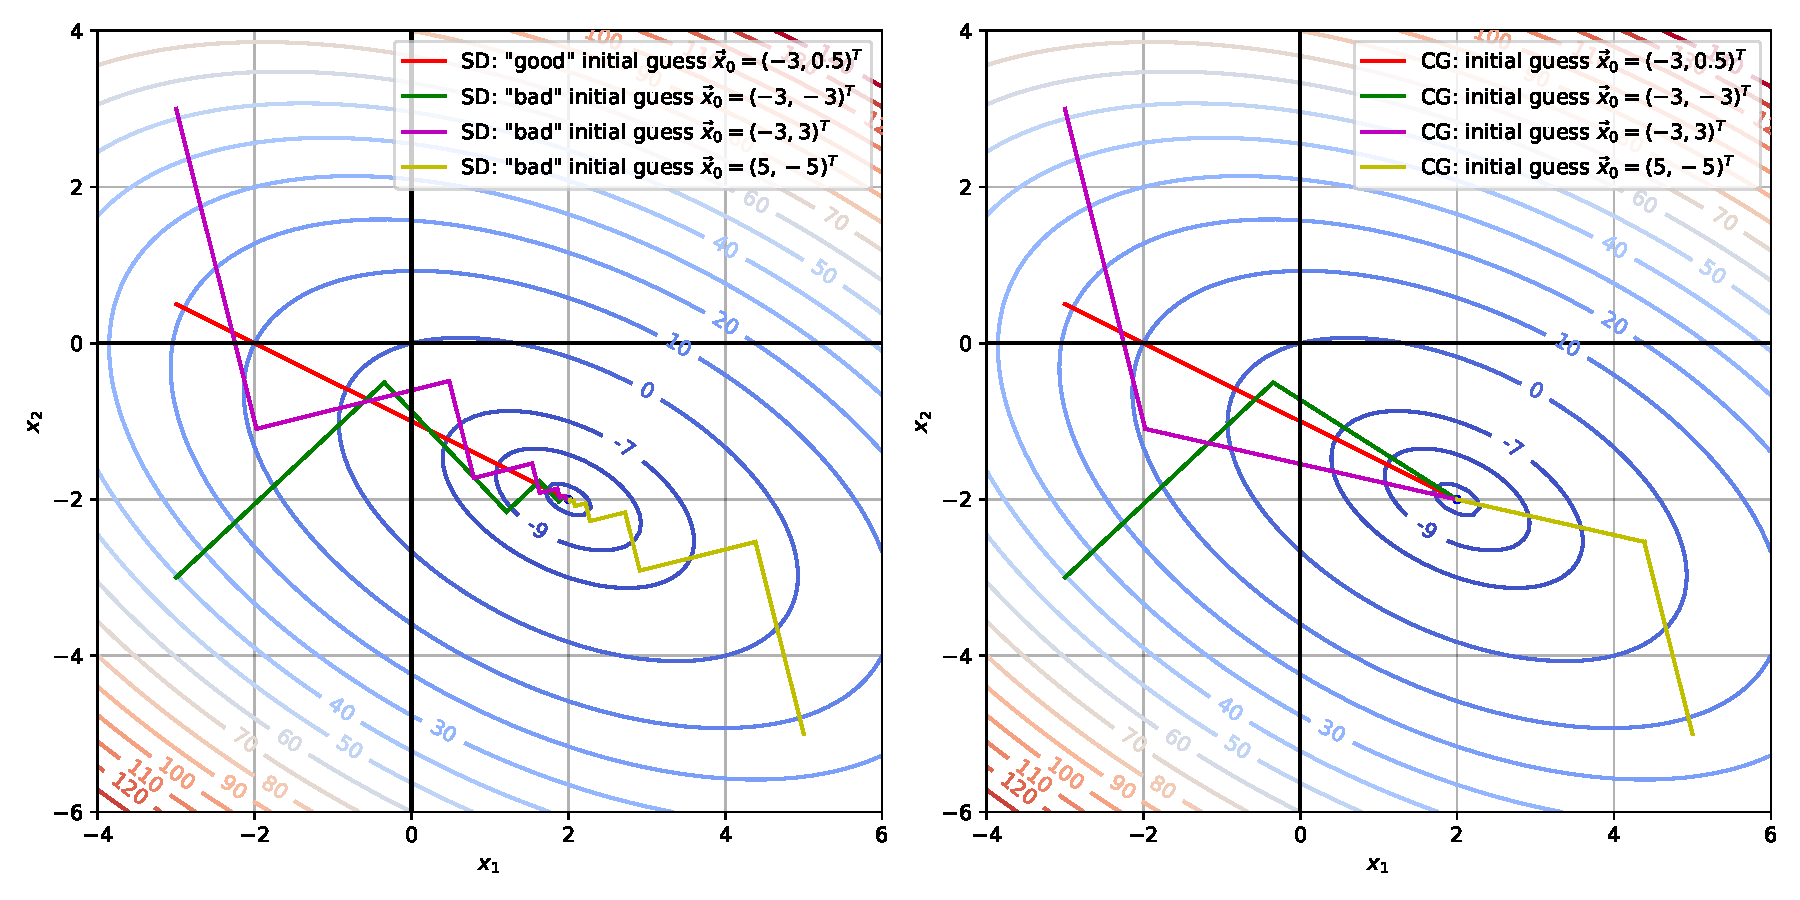
\includegraphics[width=8cm]{plots/qform_contour}
    \caption{Quandratic form TODO}
    \label{fig:qform}
\end{figure}

\begin{lemma}[Uniqueness of the solution]
The solution $\vec{x}$ in equation \eqref{eq:Axb} is unique and the global minimum of $f(\vec{x})$ if $A$ is Hermitian and positive definite \footnotemark.
\end{lemma}

\footnotetext{Notice that, negative definiteness is sufficient as well and $\vec{x}$ would be the global maximum instead - just define $A^{\prime} = -A$ which is positive definite and all of the argumentation that follows will hold as well. Indefinite matrices on the other hand might have local minima and maxima.}

\begin{proof}
Let us rewrite $f(\vec{p})$ at an arbitrary point $\vec{p} \in \mathbb{C}$ in terms of the solution vector $\vec{x}$:

\begin{align*}
    f(\vec{p}) = f(\vec{x}) + \frac{1}{2} (\vec{p} - \vec{x})^{\dagger} A (\vec{p} - \vec{x}). \numberthis \label{eq:fp_cgne}
\end{align*}

This is indeed the same as $f(\vec{p})$ (inserting $A \vec{x} = \vec{b}$ and using $A^{\dagger}=A$ and of $\vec{a}^{\dagger} \vec{b} = \vec{b}^{\dagger} \vec{a}$),

\begin{align*}
f(\vec{x}) + \frac{1}{2} (\vec{p} - \vec{x})^{\dagger} A (\vec{p} - \vec{x}) &= \frac{1}{2} \vec{x}^{\dagger} A \vec{x} - \vec{b}^{\dagger} \vec{x} + c + \frac{1}{2} \vec{p}^{\dagger} A \vec{p} - \frac{1}{2} \vec{p}^{\dagger} A \vec{x} - \frac{1}{2} \vec{x}^{\dagger} A \vec{p} + \frac{1}{2} \vec{x}^{\dagger} A \vec{x} \\
&= \frac{1}{2} \vec{p}^{\dagger} A \vec{p} + c + \vec{x}^{\dagger} \vec{b} - \vec{b}^{\dagger} \vec{x} - \vec{b}^{\dagger} \vec{p} \\
&= \frac{1}{2} \vec{p}^{\dagger} A \vec{p} - \vec{b}^{\dagger} \vec{p} + c \\
&= f(\vec{p}).
\end{align*}

In the new form of $f(\vec{p})$, one can directly see that if $A$ is positive definite, $\vec{x}$ must minimize the function:

\begin{align*}
    f(\vec{p}) = f(\vec{x}) + \frac{1}{2} \underbrace{ (\vec{p} - \vec{x})^{\dagger} A (\vec{p} - \vec{x}) }_{\text{$> 0$ if $A$ pos. def.}}.
\end{align*}

Therefore $\vec{x}$ is the global unique minimum.

\end{proof}

TODO: figure of a pos/neg definite quadratic form.

Before deriving the conjugate gradient method, we look at a related method called the \df{method of steepest descent}. We are interested in a method that iteratively solves equation \eqref{eq:Axb} starting at a \df{initial guess} $\vec{x}_0$ until the series is interrupted, because the approximate solution $\vec{x}_i$ might be close to the real solution by a certain tolerance or the solution was found exactly,

\begin{align*}
    \vec{x}_0 \longrightarrow \vec{x}_1 \longrightarrow \dotsb \longrightarrow \vec{x}_i \longrightarrow \vec{x}_{i+1} \longrightarrow \dotsb
\end{align*}

For each step, we can define the \df{error} and \df{residual} of the current step $i$.

\begin{definition}[Error and Residual]

Define the \df{error} $\vec{e}_i$ and the \df{residual} $\vec{r}_i$ as

\begin{subequations}
    \begin{align}
        \vec{e}_i &= \vec{x}_i - \vec{x}, \label{eq:error} \\
        \vec{r}_i &= \vec{b} - A \vec{x}_i. \label{eq:residual}
    \end{align}
\end{subequations}

\end{definition}

The residual is the vector of discrepancies and the same as $\vec{r}_i = -f'(\vec{x}_i) = -A \vec{e}_i$, the negative derivative of the quadratic form. The derivative point ni direction of the maximum increase, thus the residual points in direction of the steepest descent seen from the position of point $\vec{x}_i$.

\begin{definition}[Method of Steepest Descent]
The iteration step equation of the \df{method of steepest descent} in defined as

\begin{align}
    \vec{x}_{i+1} = \vec{x}_i + \alpha_i \vec{r}_i \label{eq:steepest_descent},
\end{align}

where the $\alpha_i \in \mathbb{C}$ are the amounts to go in direction $\vec{r}_i$. The $\alpha_i$ are determined by minimizing the parabola with respect to $\alpha_i$, $\frac{d}{d \alpha_i} f(\vec{x}_{i+1}) \stackrel{!}{=} 0$.

\end{definition}

TODO: figure of steepest descent zigzac.

\begin{remark}[Convergence]
As seen in figure [TODO], the method of steepest descent converges very slowly to the actual solution, when starting at a unfavorable starting point $\vec{x}_0$. The speed of convergence also heavily depends on the condition number of matrix $A$. We see that the iteration goes in the same direction multiple times. How about, when we only go \textit{once} in each direction $i$, but by the perfect amount $\alpha_i$? Then we would be done after at most $n$ steps.
\end{remark}

This gives motivation for a enhanced method. Let's define a new \df{step equation} as

\begin{align}
    \vec{x}_{i+1} = \vec{x}_i + \alpha_i \vec{p}_i, \label{eq:cg_step}
\end{align}

with \df{directions} $\vec{p}_i$ and \df{amounts} $\alpha_i$ that have to be determined. But this time, we will impose the condition to go in every direction only once at most. This will lead us to the \df{method of conjugate gradient}.

Using the step equation \eqref{eq:cg_step}, we can update the error and residuals,

\begin{subequations}
    \begin{align}
        \vec{e}_{i+1} &= \vec{x}_{i+1} - \vec{x} \\
                      &= \vec{e}_{i} + \alpha_i \vec{p}_{i} \label{eq:cg_error1} \\
                      &= \vec{e}_{0} + \sum_{j=0}^{i} \alpha_j \vec{p}_{j}, \label{eq:cg_error2}
    \end{align}
\end{subequations}

\begin{subequations}
    \begin{align}
        \vec{r}_{i+1} &= \vec{b} - A \vec{x}_{i+1} \label{eq:residual_exact} \\
                      &= \vec{r}_{i} - \alpha_i A \vec{p}_{i} \label{eq:residual_recursive} \\
                      &= - A \vec{e}_{i+1}. \label{eq:cg_error2}
    \end{align}
\end{subequations}

The $\{\vec{p}_i\}$ need to form a basis of $\mathbb{C}^n$, because the method should succeed with any arbitrary initial guess $\vec{x}_0$. Since we move in the vector space $\mathbb{C}^n$ from an arbitrary point $\vec{x}_0$ to the solution $\vec{x}$, the $n$ direction vectors need cover all possible directions in the space, therfore need to be linear independent.

To be done after at most $n$ steps, we need that the $n$-th error is zero, $\vec{e}_n = 0$. Since the directions form a basis, we can write $\vec{e}_0$ as a linear combination of the $\{\vec{p}_i\}$,

\begin{align*}
    \vec{e}_{0} = \sum_{j=0}^{n-1} \delta_j \vec{p}_j.
\end{align*}

Using this we can rewrite $\vec{e}_n$,

\begin{align*}
    \vec{e}_{n} &= \vec{e}_o + \sum_{j=0}^{n-1} \alpha_j \vec{p}_j \\
                &= \sum_{j=0}^{n-1} \delta_j \vec{p}_j + \sum_{j=0}^{n-1} \alpha_j \vec{p}_j \\
                &= \sum_{j=0}^{n-1} (\delta_j + \alpha_j) \vec{p}_j.
\end{align*}

In order for this to be zero, all coefficients need to be zero, thus $\delta_j = - \alpha_j$. Then the $i$-th error can be written in a different way

\begin{align*}
    \vec{e}_{i} &= \vec{e}_0 + \sum_{j=0}^{i-1} \alpha_j \vec{p}_j \\
                &= \sum_{j=0}^{n-1} \delta_j \vec{p}_j - \sum_{j=0}^{i-1} \delta_j \vec{p}_j \\
                &= \sum_{j=i}^{n-1} \delta_j \vec{p}_j. \numberthis \label{eq:error_i}
\end{align*}

In the last row, we can see that after every step in the iteration, we shave off the contribution of one direction $\vec{p}_i$ to the initial error $\vec{e}_0$ (or phrased differently: $\vec{e}_{i+1}$ has no contribution from direction $\vec{p}_i$). But we still need to find these directions. We could for example impose that the $(i+1)$-th error should be orthogonal to the $i$-th direction, because we never want to go in that direction again,

\begin{align*}
    0 &\stackrel{!}{=} \vec{p}_i^{\dagger} \vec{e}_{i+1} \\
                    &= \vec{p}_i^{\dagger} ( \vec{e}_{i} + \alpha_i \vec{p}_i ).
\end{align*}

This gives us a expression for the amount $\alpha_i$,

\begin{align*}
    \alpha_i = - \frac{ \vec{p}_i^{\dagger} \vec{e}_{i} }{ \vec{p}_i^{\dagger} \vec{p}_i }.
\end{align*}

The problem with this expression is that we don't know the value of $\vec{e}_i$ - if we would, we could just subtract it from the current $\vec{x}_i$ and obtain $\vec{x}$ exactly. So, we do not know $\vec{e}_i$, but what we actually know is something similar, namely $-A \vec{e}_i$, with is the residual. So if we manage to sandwich an $A$ in the expression above, we are save. It turns out that imposing $A$-orthogonality instead of regular orthogonality between $\vec{e}_{i+1}$ and $\vec{p}_i$ achieves what we're up to by the exact same steps\footnotemark,

\begin{align*}
    0 &\stackrel{!}{=} \vec{p}_i^{\dagger} A \vec{e}_{i+1} \\
                    &= \vec{p}_i^{\dagger} A ( \vec{e}_{i} + \alpha_i \vec{p}_i ) \\
\end{align*}

\footnotetext{This is equivalent to imposing $0 \stackrel{!}{=} \vec{r}_{i+1}^{\dagger} \vec{p}_i$ which is done in most literature, but in the opinion of the author this is less intuitive.}

Solving for $\alpha_i$ gives the (almost) final expression for the amounts,

\begin{align}
      \implies         \alpha_i &= - \frac{ \vec{p}_i^{\dagger} A \vec{e}_{i} }{ \vec{p}_i^{\dagger} A \vec{p}_i } = \frac{ \vec{p}_i^{\dagger} \vec{r}_{i} }{ \vec{p}_i^{\dagger} A \vec{p}_i }. \label{eq:cgne:alpha_pre}
\end{align}

Notice that the denominator is never zero, because $A$ is positive definite. Let us continue with the expression for $A$-orthoginality, but insert the derived expression \eqref{eq:error_i} for $\vec{e}_{i+1}$ this time,

\begin{align*}
    0 &\stackrel{!}{=} \vec{p}_i^{\dagger} A \vec{e}_{i+1} \\
                    &= \vec{p}_i^{\dagger} A \left[ \sum_{j=i+1}^{n-1} \delta_j \vec{p}_j \right] \\
                    &= \sum_{j=i+1}^{n-1} \underbrace{ \delta_j }_{\text{\makebox[0pt]{$\neq 0$} }} \vec{p}_i^{\dagger} A \vec{p}_j.
\end{align*}

This implies that for $j>i$ and $i \in \{0, \dots, n-1\}$, we have

\begin{align*}
    \vec{p}_i^{\dagger} A \vec{p}_j = 0.
\end{align*}

But since $A$ is Hermitian, we can Hermitian conjugate the whole expression above and obtain

\begin{align*}
    0 = \left( \vec{p}_i^{\dagger} A \vec{p}_j \right)^{\dagger} = \vec{p}_j^{\dagger} A \vec{p}_i.
\end{align*}

So the expression holds for $i>j$ as well, which implies that the $\{\vec{p}_i\}$ are \df{$A$-orthogonal},

\begin{align*}
    \vec{p}_i^{\dagger} A \vec{p}_j = 0 \quad \forall i \neq j.
\end{align*}

So the problem has reduced to finding a set of $A$-orthogonal vectors in an iterative way. Luckily there is a well know method to find orthogonal vectors from a set of linear independent vectors: \df{Gram-Schmidt orthogonalisation}. The procedure can be altered to find $A$-orthogonal vectors instead.

\begin{definition}[Gram-Schmidt Orthogonalisation]

\label{df:gramschmidt}

Let $\{ \vec{u}_0, \dots, \vec{u}_{n-1} \} \subset \mathbb{C}^n$ be a set of $n$ linear independent vectors. The iterative Gram-Schmidt procedure is

\begin{align}
    \begin{split}
        \vec{p}_0 &= \vec{u}_0 \label{eq:gramschmidt} \\
        \vec{p}_i &= \vec{u}_i + \sum_{k=0}^{i-1} \beta_{ik} \vec{p}_k,
    \end{split}
\end{align}

where the $\beta_{ik} \in \mathbb{C}$ are (to be determined) coefficients. In the regluar procedure, the $\beta_{ik}$ are just normalized projections of $\vec{u}_i$ to $\vec{p}_k$ that are subtracted from $\vec{u}_i$, leading to a vector $\vec{p}_i$ that is orthogonal to all previously calculated $\vec{p}_k$.

\end{definition}

In our problem, we need a set of vectors that are $A$-orthogonal. By imposing this condition we find a different expression for the $\beta_{ik}$,

\begin{align*}
    0 &\stackrel{!}{=} \vec{p}_i^{\dagger} A \vec{p}_j \\
                    &= \vec{u}_i^{\dagger} A \vec{p}_j + \sum_{k=0}^{i-1} \beta_{ik} \vec{p}_k^{\dagger} A \vec{p}_j \\
                    &= \vec{u}_i^{\dagger} A \vec{p}_j + \beta_{ij} \vec{p}_j^{\dagger} A \vec{p}_j,
\end{align*}

where in the last step, we assumed $i>j$ (else we would not find a expression for $\beta_{ij}$) and therefore only the $j$-th term in the sum remains, because of the $A$-orthonormality of the directions. Solving this for $\beta_{ij}$ gives

\begin{align}
    \beta{ij} = - \frac{ \vec{u}_i^{\dagger} A \vec{p}_j }{ \vec{p}_j^{\dagger} A \vec{p}_j }. \label{eq:betas}
\end{align}

In principle we are done here, we only need a set of linearly independent vectors $\{\vec{u}_i\}$. Since the conjugate gradient method is iterative and often dealing with huge problem sizes $n$, we need to store all previous directions $\vec{p}_k$ in order to calculate the current direction (see equation \eqref{eq:gramschmidt}). This becomes a problem in limited memory situations. We want that the current step only depends on the previous one. By imposing this condition, we need the sum in equation \eqref{eq:gramschmidt} to collapse; the $\beta_{ik}$ should only be non-zero for $k=i-1$. If we manage to satisfy this, the orthogonalisation procedure would simplify to

\begin{align*}
    \beta_i &\coloneqq \beta_{i, i-1}, \\
    \vec{p}_i &= \vec{u}_i + \beta_i \vec{p}_{i-1},
\end{align*}

where in the second equation, the current $\vec{p}_i$ only depends on the previous $\vec{p}_{i-1}$. For this to hold, all other $\beta_{ij}$ need to be zero. For such a $\beta_{ij}$ the numerator needs to be zero. Let therefore $j<i-1$

\begin{align*}
    \vec{u}_i^{\dagger} A \vec{p}_j &\stackrel{!}{=} 0.
\end{align*}

To find a different expression for the left hand side, consider

\begin{align*}
    \vec{u}_i^{\dagger} \vec{r}_{j+1} &= \vec{u}_i^{\dagger} \left( \vec{r}_j + \alpha_j A \vec{p}_j \right) \\
    &= \vec{u}_i^{\dagger} \vec{r}_j + \alpha_j \textcolor{cyellow}{\vec{u}_i^{\dagger} A \vec{p}_j}, \\
    \implies \textcolor{cyellow}{\vec{u}_i^{\dagger} A \vec{p}_j} &= \frac{1}{\alpha_j} \left[ \vec{u}_i^{\dagger} \vec{r}_{j+1} - \vec{u}_i^{\dagger} \vec{r}_j \right], \numberthis \label{eq:uiAdj}
\end{align*}

where we inserted the recursive relation of the resuduals \eqref{eq:residual_recursive} and the \textcolor{cyellow}{yellow} part is the expression we want to be \textcolor{cyellow}{zero} for $j<i-1$. We therefore find a condition for the linear independent set $\{\vec{u}_i\}$, namely that the scalar product of $\vec{u}_i$ with $\vec{r}_{j+1}$ and $\vec{r}_{j}$ must be the same. But we can apply the same equation over and over again and obtain

\begin{align*}
    \vec{u}_i^{\dagger} \vec{r}_{j+1} &= \vec{u}_i^{\dagger} \vec{r}_j = \dots = \vec{u}_i^{\dagger} \vec{r}_0, &j<i-1
\end{align*}

We have to find $\{\vec{u}_i\}$ that satisfy the above equation. It is sufficient to find a set of $\{\vec{u}_i\}$ that are orthogonal to all the residuals and the equation would be obeyed.

\begin{lemma}[]
\label{lem:rorthogonality}
The residuals are orthogonal, thus for all $i \neq j$, it holds

\begin{align*}
    \vec{r}_i^{\dagger} \vec{r}_j = 0.
\end{align*}

\end{lemma}

\begin{proof}

The proof consists of 2 steps.

\begin{enumerate}[label={\arabic*)}]
    \item Let $i<j$,

    \begin{align*}
        \vec{p}_i^{\dagger} \vec{r}_j &= - \vec{p}_i^{\dagger} A \vec{e}_j \\
                                      &= - \sum_{k=j}^{n-1} \delta_j \textcolor{cyellow}{\vec{p}_i A \vec{p}_k} \\
                                      &= 0,
    \end{align*}

    where the \textcolor{cyellow}{yellow} expression is \textcolor{cyellow}{zero}, because $i<j\leq k$.

    \item Let $i<j$. By step 1), we have

    \begin{align*}
        0 &= \vec{p}_i^{\dagger} \vec{r}_j \\
          &= \vec{r}_i^{\dagger} \vec{r}_j + \sum_{k=0}^{i-1} \beta_{ik} \textcolor{cyellow}{\vec{p}_k^{\dagger} \vec{r}_j} \\
          &= \vec{r}_i^{\dagger} \vec{r}_j.
    \end{align*}

    The \textcolor{cyellow}{yellow} expression is again \textcolor{cyellow}{zero} by step 1). Using the symmetry of the scalar product, the above equation also holds for $i$ and $j$ interchanged ($i>j$), therfore holds for all $i \neq j$.

\end{enumerate}

\end{proof}

From now on we set $\vec{u}_i = \vec{r}_i$. What remains to find is the final expression for the $\beta_i$.

\begin{align*}
    \beta_i \coloneqq \beta_{i,i-1} &= - \frac{ \vec{u}_i^{\dagger} A \vec{p}_{i-1} }{ \vec{p}_{i-1}^{\dagger} A \vec{p}_{i-1} } \\
    &= - \frac{1}{\vec{p}_{i-1}^{\dagger} A \vec{p}_{i-1} } \frac{1}{\alpha_{i-1}} \left[ \vec{r}_i^{\dagger} \vec{r}_i - \textcolor{cyellow}{\vec{r}_i^{\dagger} \vec{r}_{i-1}} \right] \\
    &= - \frac{ \vec{r}_i^{\dagger} \vec{r}_i }{ \alpha_{i-1} \vec{p}_{i-1}^{\dagger} A \vec{p}_{i-1} } \\
    &= - \frac{ \vec{r}_i^{\dagger} \vec{r}_i }{ \vec{p}_{i-1}^{\dagger} \vec{r}_{i-1} },
\end{align*}


where in the first row we used the definition \eqref{eq:betas}, in the second row we have used equation \eqref{eq:uiAdj} and the \textcolor{cyellow}{yellow} expression is \textcolor{cyellow}{zero} by the orthogonality of the residuals lemma \ref{lem:rorthogonality}. In the last line we used the expression for the $\alpha_j$ equation \eqref{eq:cgne:alpha_pre}

To obtain the final form of the $\alpha_i$ and the $\beta_i$, we can use a leftover of the proof of lemma \ref{lem:rorthogonality}, namely

\begin{align*}
    \vec{p}_i^{\dagger} \vec{r}_i &= \vec{r}_i^{\dagger} \vec{r}_i + \beta_i \underbrace{\textcolor{cyellow}{\vec{p}_{i-1}^{\dagger} \vec{r}_i}}_{ \mathrlap{\text{$=0$ by lemma \ref{lem:rorthogonality} step 1) }} } \\
    &= \vec{r}_i^{\dagger} \vec{r}_i.
\end{align*}


Using this we find the final form of the $\alpha_i$ and the $\beta_i$ as well as the \df{method of conjugate gradient}.

\begin{definition}[Method of conjugate gradient]

The iteration step equation of the \df{method of conjugate gradient} in defined as

\begin{align*}
    \vec{x}_{i+1} = \vec{x}_i + \alpha_i \vec{p}_i,
\end{align*}

with

\noindent\begin{minipage}{.5\linewidth}
    \begin{align*}
        \vec{r}_{i+1} &= \vec{r}_{i}   - \alpha_i A  \vec{p}_i, \\
        \vec{p}_{i+1} &= \vec{r}_{i+1} + \beta_{i+1} \vec{p}_i, 
    \end{align*}
\end{minipage}
\begin{minipage}{.5\linewidth}
    \begin{align}
        \alpha_i    &=   \frac{ \vec{r}_{i}^{\dagger} \vec{r}_{i} }{ \vec{p}_i^{\dagger} A \vec{p}_i }, \label{eq:alphai} \\
        \beta_{i+1} &= - \frac{ \vec{r}_{i+1}^{\dagger} \vec{r}_{i+1} }{ \vec{r}_{i}^{\dagger} \vec{r}_{i} }, \label{eq:betai}
    \end{align}
\end{minipage}

and initial starting vectors

\begin{align*}
    \vec{x}_{0} &= \text{arbitrary starting point}, \\
    \vec{p}_{0} &= \vec{r}_{0} = \vec{b} - A \vec{x}_0.
\end{align*}

\end{definition}

There are some remarks to note about the method of conjugate gradient.

\begin{remark}
    The $\beta_{i+1}$ of the current iteration depends on the norm of the current residual as well as the last one. This means that we can store the result of the last iteration and reuse it in the current, the norm may not be calculated twice.
\end{remark}

\begin{remark}
    In the souce code of openQxD (see \cite{openqxd}) the matrix $A$ is the Dirac matrix applied twice $A = D^{\dagger} D$. This means that the denominator of $\alpha_i$ is a regular inner product as well; $\vec{p}_i^{\dagger} A \vec{p}_i = \vec{p}_i^{\dagger} D^{\dagger} D \vec{p}_i = \left( D \vec{p}_i \right)^{\dagger} \left( D \vec{p}_i \right) = \norm{ D \vec{p}_i }^2$
\end{remark}

\begin{remark}
    Therefore in each iteration, we have:
    \begin{itemize}
        \item 2 times the norm of a vector,
        \item 2 matrix-vector multiplications,
        \item 3 times axpy.\footnotemark
    \end{itemize}
\end{remark}

\begin{remark}[Floating point errors]
    Since the method contains recursive steps, floating point roundoff accumulation is an issue. This causes the residuals to loose their $A$-orthogonality. It can be resolved by calculating the residual from time to time using its (computationally more expensive) definition $\vec{r}_i = \vec{b} - A \vec{x}_i$, which involves one matrix vector multiplication. One can for example do this every $m$-th step. The same problem applies to the directions $\vec{p}_i$ that loose their $A$-orthogonality.
\end{remark}

\begin{remark}[Problem size]
    The method of conjugate gradient is suitable for problems of very huge size $n$. The algorithm is done after $n$ steps, but there might be problems such that even $n$ steps are out of reach for an exact solution.
\end{remark}

\begin{remark}[Complexity]
    The time complexity of the conjugate gradient method is $O(m \sqrt{\kappa})$, where $m$ is the number of non-zero entries in $A$ and $\kappa$ is its \df{condition number}. The space complexity is $O(m)$.
\end{remark}

\begin{remark}[Starting]
    The \df{starting vector} $\vec{x}_0$ can be chosen at wish. If there is already a rough estimate of the solution one can take that vector. But usually just $\vec{x}_0 = 0$ is chosen. Since the minimum is global, there is no issue in chosing a starting point. The method will always converge towards the real solution.
\end{remark}

\begin{remark}[Stopping]
    If the problem size does not allow to run $n$ steps, one can stop when the norm of the residual falls below a certain \df{threshold} value. Usually this threshold is a fraction of the initial residual $\norm{\vec{r}_i} < \epsilon \norm{\vec{r}_0}$ \cite{shewchuk1994}.
\end{remark}

\begin{remark}[Initialization]
    The very first step of the method is equivalent to a step in the method of steepest descent, see equation \eqref{eq:steepest_descent}.
\end{remark}

\begin{remark}[Speed of convergence]
    TODO: cg is quicker if there are duplicated eigenvalues. number of iterations for exact solution is at most the number of distinct eigenvalues.
\end{remark}

\begin{remark}[Preconditioning]
    The linear system of equations can be transformed using a matrix $M$ to

    \begin{align*}
        M^{-1} A \vec{x} = M^{-1} \vec{b}.
    \end{align*}

    It is assumed $M$ is such that is is easy to insert and it approximates $A$ in some way, resulting in $M^{-1} A$ to be better conditioned than was $A$. An examples of a particular preconditioner $M$ would be a diagonal matrix, with diagonal entries of $D$. It is indeed easy to invert and it approximates $A$ quite well if $A$ has non-zero diagonal entries and most off-diangonal entries are zero.
\end{remark}

\begin{remark}[\acrfull{cgne}]
    The algorithm can be used even if $A$ is not symmetric nor Hermitian nor positive definite. The linear system of equations to be solved is then

    \begin{align*}
        A^{\dagger} A \vec{x} = A^{\dagger} \vec{b}.
    \end{align*}

    If $A$ is square and invertible, solving the above equation is equivalent to solving $A \vec{x} = \vec{b}$. Conjugate gradient can be applied, because $A^{\dagger} A$ is Hermitian and positive ($\vec{x}^{\dagger} A^{\dagger} A \vec{x} = \norm{A \vec{x}} \ge 0$). Notice that $A^{\dagger} A$ is less sparse than $A$, and often $A^{\dagger} A$ is bady conditioned.

\end{remark}

\footnotetext{This stands for $a \vec{x} + \vec{y}$, scalar times vector plus vector, "a x plus y" (to resemble the \acrshort{BLAS} level 1 routine call of the same name).}

\section{Real number formats}
\label{sec:floats}

\subsection{IEEE Standard for Floating-Point Arithmetic}

Floating point numbers are omnipresent in the scientific applications. In the conjugate gradient kernel of \cite{openqxd}, there are large scalar products over vectors of very high dimensionality over multiple ranks. The components of these vectors are single precision floating point numbers (I call them \gls{binary32} from here on). The precision was degraded from \gls{binary64} to \gls{binary32} already and a speedup of a factor of 2 was achieved. This motivates to explore even smaller floating point formats with encoding lengths of 16 bits. Since scalar products as well as matrix-vector products are memory-bound operations, going to a smaller bit-length will increase the throughput of the calculation. Therefore, a 16 bits floating point format with a smaller exponent could lead to a double of performance if the new operation is still memory-bound.

\begin{definition}[IEEE 754 Floating point format]

The \df{IEEE 754 floating point format} \cite{ieee754_1985} is defined using the \df{number of exponent bits} $e$ and the \df{number of mantissa bits} $m$ respectivetly. A binary floating point number is illustrated in Figure \ref{fig:float}.

\begin{figure}[H]
  \includestandalone[width=\textwidth]{schemes/float}
  \caption{Binary representation of a IEEE 754 $n$-bit precision floating-point number. The \textcolor{corange}{orange} bit represents the \textcolor{corange}{sign bit}, the \textcolor{cblue}{blue} bits represent the fixed-length \textcolor{cblue}{e exponent bits} and the \textcolor{cgreen}{green} bits represent the fixed-length \textcolor{cgreen}{m mantissa bits}. Notice that $n = \textcolor{corange}{1} + \textcolor{cblue}{e} + \textcolor{cgreen}{m}$.}
  \label{fig:float}
\end{figure}

\end{definition}

The resulting floating point number is then calculated as

\begin{align*}
    f = (-1)^{\textcolor{corange}{s}} \cdot \textcolor{cgreen}{M} \cdot 2^{\textcolor{cblue}{E}},
\end{align*}

where $E=E^{\prime}-B$ denotes the biased exponent, $B$ is the exponent bias, $M$ the mantissa and $s$ the sign bit. The (unbiased) exponent $E^{\prime}$ is calculated as follows

\begin{align}
    E^{\prime} = \sum_{i=0}^{(e-1)} b_{m+i} 2^i, \label{eq:exponent}
\end{align}

where $B$ is the exponent bias.

\begin{definition}[Exponent bias]

\begin{align*}
    B = 2^{(e-1)} -1,
\end{align*}

\end{definition}

The calculation of the mantissa is a bit more involved, since it depends on the number being normal or subnormal.

\begin{definition}[Subnormal numbers]

The IEEE 754 standard introduces so called \df{subnormal numbers}. If all the exponent bits are $0$, meaning the unbiased exponent $E^{\prime}=0$, and the mantissa bits are not all $0$, then the number is called subnormal. The exponent being zero causes the implcit bit to flip to $0$, instead of $1$.

\end{definition}

\begin{remark}
    Subnormal numbers have a variable-length mantissa and exponent, because some of the mantissa bits are used as additional exponent bits, making the numbers less precise the lower they get (see the smooth cutoff in Figure \ref{fig:number_line}).
\end{remark}

Therefore the mantissa of a regular (non-subnormal) number is (when the exponent $0<E<B$, this implies that the implicit bit is $1$)

\begin{align*}
    M = \tikzmark{implicit1}\textcolor{cyellow}{1} + \sum_{i=1}^{m} b_{m-i} 2^{-i},
\end{align*}

\begin{tikzpicture}[remember picture,overlay]
\draw[<-] 
  ([shift={(3pt,-2pt)}]pic cs:implicit1) |- ([shift={(-14pt,-10pt)}]pic cs:implicit1) 
  node[anchor=east] {$\scriptstyle \text{implicit bit}$}; 
\end{tikzpicture}

whereas the mantissa of a subnormal number (when the exponent $E=0$) is

\begin{align*}
    M = \tikzmark{implicit0}\textcolor{cyellow}{0} + \sum_{i=1}^{m} b_{m-i} 2^{-i},
\end{align*}

\begin{tikzpicture}[remember picture,overlay]
\draw[<-] 
  ([shift={(3pt,-2pt)}]pic cs:implicit0) |- ([shift={(-14pt,-10pt)}]pic cs:implicit0) 
  node[anchor=east] {$\scriptstyle \text{implicit bit}$}; 
\end{tikzpicture}

The $1$ or $0$ in the front of the summand is the leading \df{\textcolor{cyellow}{implicit bit}}, sometimes also called the \df{$(m+1)$-th mantissa bit} that tells us whether the number is subnormal or not.

\begin{remark}
    The mantissa range of a regular floating point number is $M \in [1, 2)$, whereas the matissa range of a subnormal floating point number is $M \in (0, 1)$. The number zero is not considered subnormal.
\end{remark}

Usual floating point formats are summarised in Table \ref{tab:formats}.

\bgroup
\def\arraystretch{1.2}%  1 is the default, change whatever you need
\begin{table}
\centering

    \begin{tabular}{ |p{2cm}||>{\columncolor{corange!20}}p{0.3cm}|>{\columncolor{cblue!20}}p{0.6cm}|>{\columncolor{cgreen!20}}p{0.6cm}|p{6cm}|  }
        \hline
        \multicolumn{5}{|c|}{Floating point formats} \\
        \hline
        name & \textcolor{corange}{s} & \textcolor{cblue}{e} & \textcolor{cgreen}{m} & comment \\
        \hline
        \gls{binary64}  & \textcolor{corange}{1} & \textcolor{cblue}{11} & \textcolor{cgreen}{52} & double precision, IEEE 754 \cite{ieee754_2008} \\
        \gls{binary32}  & \textcolor{corange}{1} & \textcolor{cblue}{8}  & \textcolor{cgreen}{23} & single precision, IEEE 754 \cite{ieee754_2008} \\
        \gls{binary16}  & \textcolor{corange}{1} & \textcolor{cblue}{5}  & \textcolor{cgreen}{10} & half precision, IEEE 754 \cite{ieee754_2008} \\
        \gls{bfloat16}  & \textcolor{corange}{1} & \textcolor{cblue}{8}  & \textcolor{cgreen}{7} & Googles Brain Float \cite{bfloat16} \\
        \gls{tensorfloat32}      & \textcolor{corange}{1} & \textcolor{cblue}{8}  & \textcolor{cgreen}{10} & NVIDIAs TensorFloat-32 \cite{tf32} \footnotemark \\
        \hline
        binary24  & \textcolor{corange}{1} & \textcolor{cblue}{7}  & \textcolor{cgreen}{16} & AMDs fp24 \cite{fp24} \\
        binary128       & \textcolor{corange}{1} & \textcolor{cblue}{15} & \textcolor{cgreen}{112} & IEEE 754 \cite{ieee754_2008} \\
        binary256 & \textcolor{corange}{1} & \textcolor{cblue}{19} & \textcolor{cgreen}{236} & IEEE 754 \cite{ieee754_2008}\\
        \hline
    \end{tabular}
    \caption{\label{tab:formats} Commonly used floating point formats, where $s$ is the number of sign bits, $e$ the number of exponent bits and $m$ the number of mantissa bits.}
    
\end{table}
\egroup

\footnotetext{Allocates 32 bits, but only 19 bits are actually used.}

The format of interest is the \gls{binary16} half precision IEEE 754 floating point format. The highest representable number is when the exponent is highest. This is not the case when all $e$ exponent bits are $1$, because then - according to the specification \cite{ieee754_1985} - the number is either $\pm \infty$ or \acrfull{nan}, depending on the mantissa. The maximal unbiased exponent is therefore the next smaller number,

\begin{align*}
    E^{\prime}_{max} = \underbrace{ 1...1 }_{\text{\makebox[0pt]{$e-1$ times} }}0.
\end{align*}

Using equation \eqref{eq:exponent}, we find

\begin{align*}
    E^{\prime}_{max} &= \sum_{i=1}^{(e-1)} 2^i \\
            &= 2^e -2.
\end{align*}

The mantissa on the other hand is maximal when all mantissa bits are $1$ (including the implicit bit),

\begin{align*}
    M_{max} &= 1 + \sum_{i=1}^{m} 2^{-i} \\
            &= 2 - 2^{-m}.
\end{align*}

Using these two formulas we can define the

\begin{definition}[\df{highest representable number}]

The \df{highest representable number} in any floating point format is

\begin{align*}
    f_{max} &= (-1)^0 \cdot M_{max} \cdot 2^{(E^{\prime}_{max} - B)} \\
            &= ( 2 - 2^{-m} ) \cdot 2^{(2^e -2^{e-1} -1)} \\
            &= ( 2 - 2^{-m} ) \cdot 2^{(2^{e-1} -1)}.
\end{align*}

\end{definition}

The minimal number above \num{0} can be found similarly, using minimal unbiased exponent (when all exponent bits are \num{0}, except the last one, therefore $E^{\prime}_{min} = 1$) and the minimal mantissa ($M_{min} = 1$).

\begin{definition}[\df{minimal (non-subnormal) representable number above \num{0}}]

The \df{minimal (non-subnormal) representable number above \num{0}} in any floating point format is

\begin{align*}
    f_{min} &= (-1)^0 \cdot M_{min} \cdot 2^{(E^{\prime}_{min} - B)} \\
            &= 2^{(2 - 2^{e-1})}.
\end{align*}

\end{definition}

The minimal subnormal number can the found, when the unbiased exponent consists of only zeros ($E^{\prime}_{smin} = 0$) and for the mantissa, only the rightmost bit is one ($M_{smin} = 2^{1-m}$).

\begin{definition}[\df{minimal subnormal representable number above \num{0}}]

The \df{minimal subnormal representable number above \num{0}} in any floating point format is

\begin{align*}
    f_{min} &= (-1)^0 \cdot M_{smin} \cdot 2^{(E^{\prime}_{smin} - B)} \\
            &= 2^{1-m} \cdot 2^{(1 - 2^{e-1})} \\
            &= 2^{(2 -m -2^{e-1})}.
\end{align*}

\end{definition}

See Table \ref{tab:float:limits} for these limiting numbers in the different floating point formats.

\bgroup
\def\arraystretch{1.2}%  1 is the default, change whatever you need
\begin{table}
\centering

    \begin{tabular}{ |p{2cm}||p{2cm}|p{2cm}|p{2cm}|p{2cm}|  }
        \hline
        \multicolumn{5}{|c|}{Floating point format limits} \\
        \hline
        name & $f_{max}$ & $f_{min}$ & $f_{smin}$ & sign. digits \footnotemark \\
        \hline
        \gls{binary64}
            & \num[round-mode = figures, round-precision = 2, scientific-notation = true]{1.79769313486231570e308}
            & \num[round-mode = figures, round-precision = 2, scientific-notation = true]{2.22507385850720138e-308}
            & \num[round-mode = figures, round-precision = 2, scientific-notation = true]{4.94065645841246544e-324}
            & $\le 15.9$ \\
        \gls{binary32}
            & \num[round-mode = figures, round-precision = 2, scientific-notation = true]{3.402823466e38}
            & \num[round-mode = figures, round-precision = 2, scientific-notation = true]{1.175494350e-38}
            & \num[round-mode = figures, round-precision = 2, scientific-notation = true]{1.401298464e-45}
            & $\le 7.2$ \\
        \gls{binary16}
            & \num[round-mode = figures, round-precision = 2, scientific-notation = true]{65504}
            & \num[round-mode = figures, round-precision = 2, scientific-notation = true]{0.00006103515625}
            & \num[round-mode = figures, round-precision = 2, scientific-notation = true]{5.9604644625e-8}
            & $\le 3.3$ \\
        \gls{bfloat16}
            & \num[round-mode = figures, round-precision = 2, scientific-notation = true]{3.38953138e38}
            & \num[round-mode = figures, round-precision = 2, scientific-notation = true]{1.175494350e-38}
            & \num[round-mode = figures, round-precision = 2, scientific-notation = true]{9.18354961e-41}
            & $\le 2.4$ \\
        \gls{tensorfloat32}
            & \num[round-mode = figures, round-precision = 2, scientific-notation = true]{3.40116213e38}
            & \num[round-mode = figures, round-precision = 2, scientific-notation = true]{1.175494350e-38}
            & \num[round-mode = figures, round-precision = 2, scientific-notation = true]{1.14794370e-41}
            & $\le 7.2$ \\
        \hline
        binary24
            & \num[round-mode = figures, round-precision = 2, scientific-notation = true]{1.84466033e19}
            & \num[round-mode = figures, round-precision = 2, scientific-notation = true]{2.16840434e-19}
            & \num[round-mode = figures, round-precision = 2, scientific-notation = true]{3.30872245e-24}
            & $\le 5.1$ \\
        binary128
            & \num[round-mode = figures, round-precision = 2, scientific-notation = true]{1.189731495357231765085759326628007016196469052641694045529e4932}
            & \num[round-mode = figures, round-precision = 2, scientific-notation = true]{3.36210314311209350626267781732175260259807934484647124010e-4932}
            & \num[round-mode = figures, round-precision = 2, scientific-notation = true]{6.47517511943802511092443895822764655249956933803468100968e-4966}
            & $\le 34$ \\
        binary256
            & \num[round-mode = figures, round-precision = 2, scientific-notation = true]{1.61132571748576047361957211845200501064402387454966951747e78913}
            & \num[round-mode = figures, round-precision = 2, scientific-notation = true]{1e-78912}
            & \num[round-mode = figures, round-precision = 2, scientific-notation = true]{1e-78983}
            & $\le 71.3$ \\
        \hline
    \end{tabular}
    
    \caption{\label{tab:float:limits} Summary of highest representable numbers, minimal subnormal and non-subnormal representable numbers above \num{0} in any IEEE 754 floating point format together with their approximated precision.}
    
\end{table}
\egroup

\footnotetext{Number of significant digits in decimal; $-\log_{10} (\code{MACHINE\_EPSILON}) = \log_{10} (2^{m+1})$.}

\subsection{Posits}

The posit datatype is designed to be a replacement for the IEEE floating point format, fixing its various quirks. Some of the more entertaining are:

\begin{itemize}
    \item The appearance of \acrshortpl{nan}. They are considered unnatural, because a specific bit pattern describing a number that is not a number is a contradiction.
    \item The \acrshortpl{nan} and the fact that floats have two different representations for the number zero ($0$ and $-0$) lead to very complicated and slow comparison units.
    \item Floats may under- or overflow, because the standard employs the round to nearest even rounding rule ($\pm \infty$ and $0$ are considered even).
    \item Floats are non-associative and non-distributive\footnotemark leading to rounding errors that have to be taken into account, specially in scientific computing.
    \item The standard gives no guarantee of bit-identical results across systems.
\end{itemize}

\footnotetext{There was even a system using IEEE 754 that had non-commutative floating point operations\cite{cody1980}.}

The goal is to utilise the number of bits more efficiently and remove these inconsistencies. The key idea is to place half of all numbers between $0$ and $1$ and the other half are the reciprocals (the reciprocal of $0$ being $\pm \infty$). The number can then be drawn on a projective real number circle \cite{gustafson2017}. The structure of a binary posit number is illustrated in Figure \ref{fig:posit}.

\begin{figure}[H]
  \includestandalone[width=\textwidth]{schemes/posit}
  \caption{Binary representation of a $n$-bit posit number. As with regular floats the \textcolor{corange}{orange} bit represents the \textcolor{corange}{sign bit}, the \textcolor{cyellow}{yellow} bit(s) represent the variable length \textcolor{cyellow}{regime bit(s)} terminated by the \textcolor{cbrown}{brown} bit that is the \textcolor{cbrown}{opposite regime bit}, the \textcolor{cblue}{blue} bit(s) represent the variable-length \textcolor{cblue}{exponent bit(s)} and the \textcolor{cgreen}{green} bit(s) represent the variable-length \textcolor{cgreen}{mantissa bit(s)}.}
  \label{fig:posit}
\end{figure}

The actual value of the number is calculated as follows. The yellow and brown bits determine the regime of the number. They either start with a \textcolor{cyellow}{row of all \num{0} or all \num{1}} terminated by the \textcolor{cbrown}{opposite bit} indicating the end of the row. The number of bits in the row are counted as $m$ and if they are all \num{0} they get a minus sign, the regime being $k=-m$. If they are all \num{1} the regime is calculated as $k=m-1$. After the regime is decocded, the remaining bits contain the exponent with at most $es$ bits depending on how much bits remain. If no bits remain the exponent is \num{0}. The exponent and the mantissa are both of variable length. Both can have \num{0} bits, in this case the number consists of only regime bits. This is the reason why posits have a larger number range than floats. The exponent is enconded as unsigned integer, so there is no bias and no bit pattern denoting special numbers such as subnormals or \acrshortpl{nan}. Therefore $n$-bit posits have more numbers than $n$-bit floats, because they have no \acrshortpl{nan}. After the exponent - if there are still bits remaining - the fraction follows, else the fraction is just $1.0$ Since there are no subnormals the implicit bit is always \num{1}. There are two special numbers that do not follow the above encoding scheme; zero which has the bit pattern of all \num{0} and $\pm \infty$ with a \num{1} followed by all \num{0}. These two numbers are reciprocals of each other. A general posit number can therefore be written as

\begin{align*}
    p = (-1)^{\textcolor{corange}{s}} \cdot useed^{\textcolor{cyellow}{k}} \cdot \textcolor{cgreen}{M} \cdot 2^{\textcolor{cblue}{E}},
\end{align*}

where $s$ is the sign bit, $useed$ is defined to be $useed = 2^{2^{es}}$, with $es$ the number of predefined exponent bits, $M$ is the mantissa and $E$ the exponent.

The mantissa is calculated as

\begin{align*}
    M = 1 + \sum_{i=1}^{m} m_{i} 2^{m-i},
\end{align*}

where $m$ is the variable number of mantissa bits and the implicit bit in front of the sum is always \num{1}. The exponent is

\begin{align*}
    E = \sum_{i=1}^{e} e_{i} 2^{e-i},
\end{align*}

where $e$ is the variable number of exponent bits satisfying $e \le es$.

Using these two equations, we are now able to calculate the highest representable number and the minimal representable number above \num{0} in posit format.

\begin{definition}[\df{highest representable number}]

The \df{highest representable number} in any posit format is

\begin{align*}
    p_{max} &= (-1)^0 \cdot useed^{n-2} \\
            &= 2^{2^{es}(n-2)}.
\end{align*}

\end{definition}

\begin{definition}[\df{minimal representable number above \num{0}}]

The \df{minimal representable number above \num{0}} in any posit format is the reciprocal of the highest representable number $p_{max}$

\begin{align*}
    p_{min} &= \frac{1}{p_{max}} \\
            &= 2^{2^{es}(2-n)}.
\end{align*}

\end{definition}

See Table \ref{tab:posit:limits} for these limiting numbers in the different posit formats.

\bgroup
\def\arraystretch{1.2}%  1 is the default, change whatever you need
\begin{table}
\centering

    \begin{tabular}{ |p{2cm}|>{\columncolor{cblue!20}}p{0.6cm}||p{2cm}|p{2cm}|p{2cm}|  }
        \hline
        \multicolumn{5}{|c|}{Posit format limits} \\
        \hline
        name & \textcolor{cblue}{$es$} & $p_{max}$ & $p_{min}$ & sign. digits \footnotemark \\
        \hline
        \gls{posit64}
            & \textcolor{cblue}{\num{3}}
            & \num[round-mode = figures, round-precision = 2, scientific-notation = true]{2.04586912993508866875e149}
            & \num[round-mode = figures, round-precision = 2, scientific-notation = true]{4.88789818159936749128e-150}
            & $\le 17.7$ \\
        \gls{posit32}
            & \textcolor{cblue}{\num{2}}
            & \num[round-mode = figures, round-precision = 2, scientific-notation = true]{1.32922799578491587290e36}
            & \num[round-mode = figures, round-precision = 2, scientific-notation = true]{7.52316384526264005099e-37}
            & $\le 8.1$ \\
        \gls{posit16}
            & \textcolor{cblue}{\num{1}}
            & \num[round-mode = figures, round-precision = 2, scientific-notation = true]{2.68435456e8}
            & \num[round-mode = figures, round-precision = 2, scientific-notation = true]{3.72529029e-9}
            & $\le 3.6$ \\
        \gls{posit8}
            & \textcolor{cblue}{\num{0}}
            & \num{64}
            & \num[round-mode = figures, round-precision = 2, scientific-notation = true]{0.015625}
            & $\le 1.5$ \\
        \hline
    \end{tabular}
    
    \caption{\label{tab:posit:limits} Summary of highest representable numbers, minimal representable numbers above \num{0} in any posit format together with their approximated precision.}
    
\end{table}
\egroup

\footnotetext{Number of significant digits in decimal; $-\log_{10} (\code{MACHINE\_EPSILON})$. Notice that posits have \df{tapered accuracy}; numbers near \num{1} have much more precision than numbers at the borders of the regime. The precision of floats decreses as well with very large and small numbers, but posit precision decreases faster, see Figure \ref{fig:number_line}.}

Posits employ a feature called the \gls{quire}, which is the generalized answer to the \gls{fma} operation that recently found its way into \cite{ieee754_2008} in 2008, where the rounding is deferred to the very end of the operation.

\begin{figure}
    \centering
    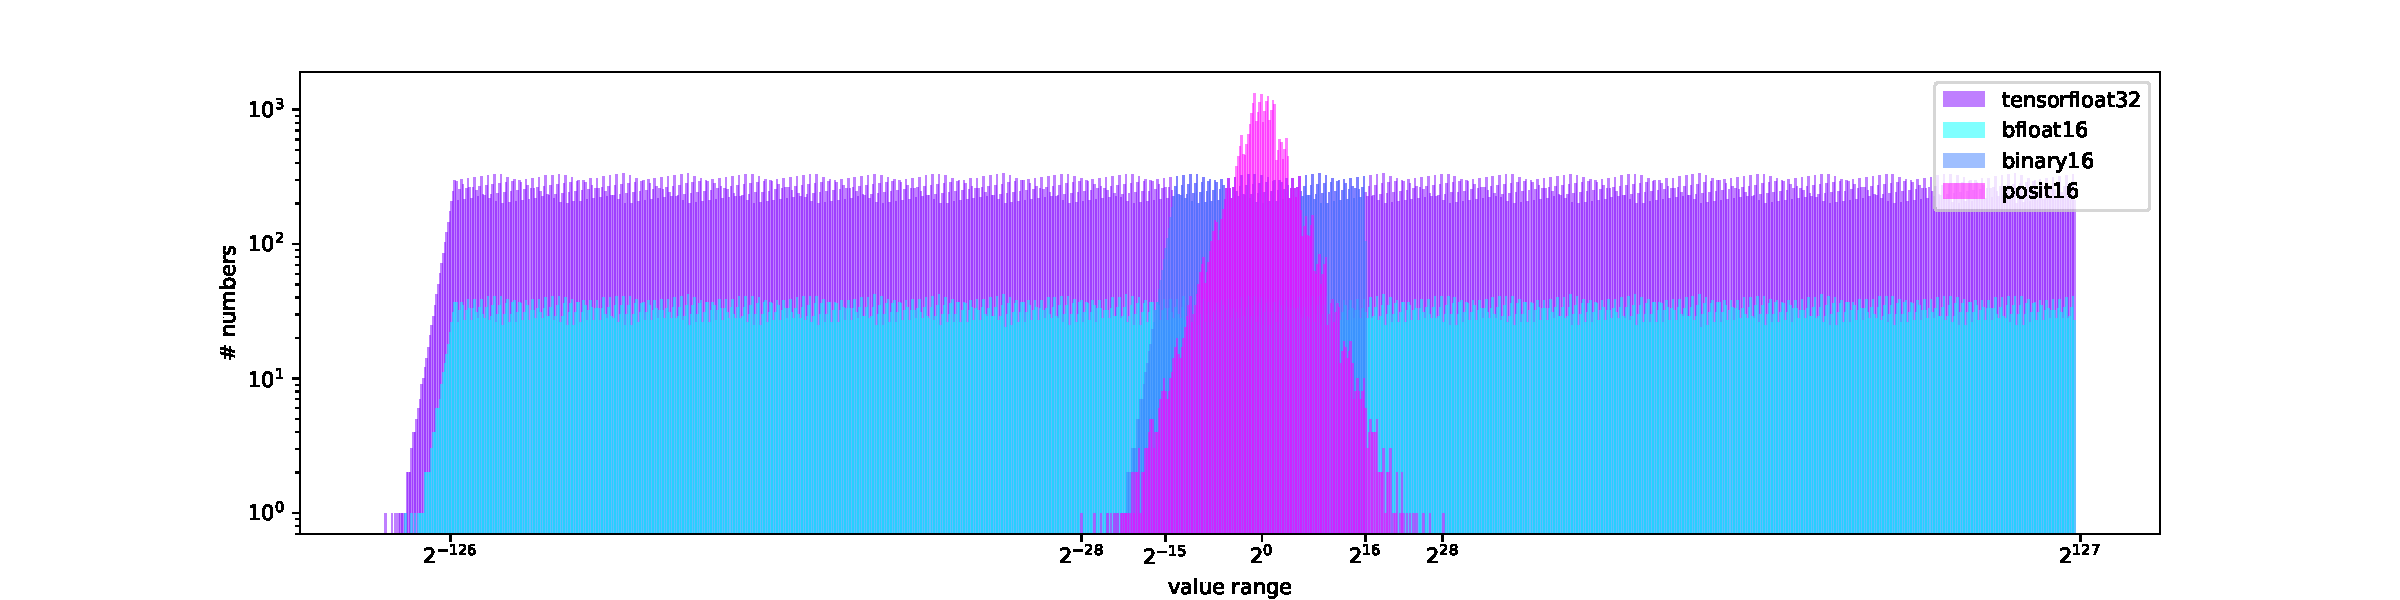
\includegraphics[width=1.0\textwidth]{plots/number_line}
    \caption{Density or distribution of numbers for \gls{tensorfloat32}, \gls{binary16}, \gls{posit16} and \gls{bfloat16}. The number of bins was chosen to be \num{1024} of logarithmic width. The IEEE conformant floats \gls{tensorfloat32}, \gls{binary16} and \gls{bfloat16} exhibit a simmilar shape, namely the distribution of numbers is exponential decreasing for higher and smaller numbers. The high numbers undergo a rough cutoff at the highest representable number. Numbers above that value will be cast to infinity. Compared to this, the small numbers show a smooth cutoff, because of the existence subnormal numbers. The range of \gls{posit16} is bigger than the range of \gls{binary16}, but specially in the very small numbers this difference in range is neglectible. Some features of posits can be observed: First, their distribution is symmetric around \num{1}, because posits have no subnormals. Second, more numbers are closer to \num{1} than in case of floats; the closer to \num{1}, the better the number resolution. Closest to \num{1}, the number resolution becomes better than \gls{binary16} resolution. Third, posits have no fixed-length mantissa nor exponent. That's the reason why the height of the posit shape depends on the number regime, which happens for floats only in the subnormal regime, where the exponent and mantissa are indeed of variable length. For all formats, the amount of numbers decreases exponentially when going away from \num{1}, but posits decrease faster. This suggests that when calculating in the number regime close to \num{1} posits might be the better choice, but when numbers span the whole number range equally, floats might be superior. But in that case one has to take care about over- and underflows. Notice that the height of the shape is determined by the number of mantissa bits, therefore giving the precision, whereas the width is determined by the number of exponent bits, therefore giving the number range. For example \gls{tensorfloat32} and \gls{binary16} have a very different number range, but exhibit the same percision for numbers in their intersection, meaning that \gls{binary16} is a subset of \gls{tensorfloat32}. On the other hand comparing \gls{tensorfloat32} and \gls{bfloat16} they have approximately the same number range, but different precisions in them, meaning that \gls{bfloat16} is as well a subset of \gls{tensorfloat32}, which itself is a subset of \gls{binary32}. Notice that when plotting \gls{binary32} and \gls{posit32} in such a plot, they would look very similar to \gls{binary16} versus \gls{posit16}.}
    \label{fig:number_line}
\end{figure}

\subsection{Floating point numbers in openQxD}

To explore how the conjugate gradient kernel in openQxD would perform when using smaller bit lengths, one can look at the exponentials of the numbers in the matrix and vectors, see Figure \ref{fig:exponents}. The plot shows all exponents appearing together with their overall occurence in percent. The number zero was taken from the plot, because it has biased exponent $E=-127$. The occurences for zero are given in the legend.

The highest exponent in all 4 runs was $E=4$, whereas the lowest exponent deceased when the number of lattice points increased. The range of exponents that is representable in \gls{binary16} spans from \textcolor{corange}{$-24$} to \textcolor{cpink}{$+16$} and is indicated by the \textcolor{corange}{solid orange line} and the \textcolor{cpink}{solid pink line}. Between \textcolor{corange}{$-24$} and \textcolor{cblue}{$-14$} is the regime of subnormal numbers in \gls{binary16}, with the lowest regular (non-subnormal) exponent indicated by the \textcolor{cblue}{solid blue line}. When using half precision instead of single precision, all numbers with exponents below \textcolor{corange}{$-24$}, will be converted to zero, whereas exponents above \textcolor{cpink}{$+16$} will be casted to $\pm \infty$ depending on the sign of the number. It can be seen, that when calculating the norm of these numbers, only numbers between the \textcolor{cblue}{dashed blue line} and the \textcolor{cpink}{dashed pink line} will participate. If there is a number above the dashed pink line in the \textcolor{cyellow}{unsave region} this number will - after squaring - be casted to $\infty$ and therefore the norm will be $\infty$ as well\footnotemark. In this case the variable representing the norm $x = \norm{\vec{v}}$ should be of higher precision than \gls{binary16}. The plot shows that the Dirac matrix \code{Dop()} is confined in a narrow exponent regime and a representation in 16-bit floats would suffice. Notice the sparsity the Dirac matrix.

\footnotetext{A method to circumvent this is to scale the vector entries during the calculation and scale the result back, exploiting homogeneity of the norm, $\norm{\vec{v}} = \frac{1}{s}\norm{s\vec{v}}$ for $s \in \mathbb R_{> 0}$.}

\begin{figure}
    \centering
    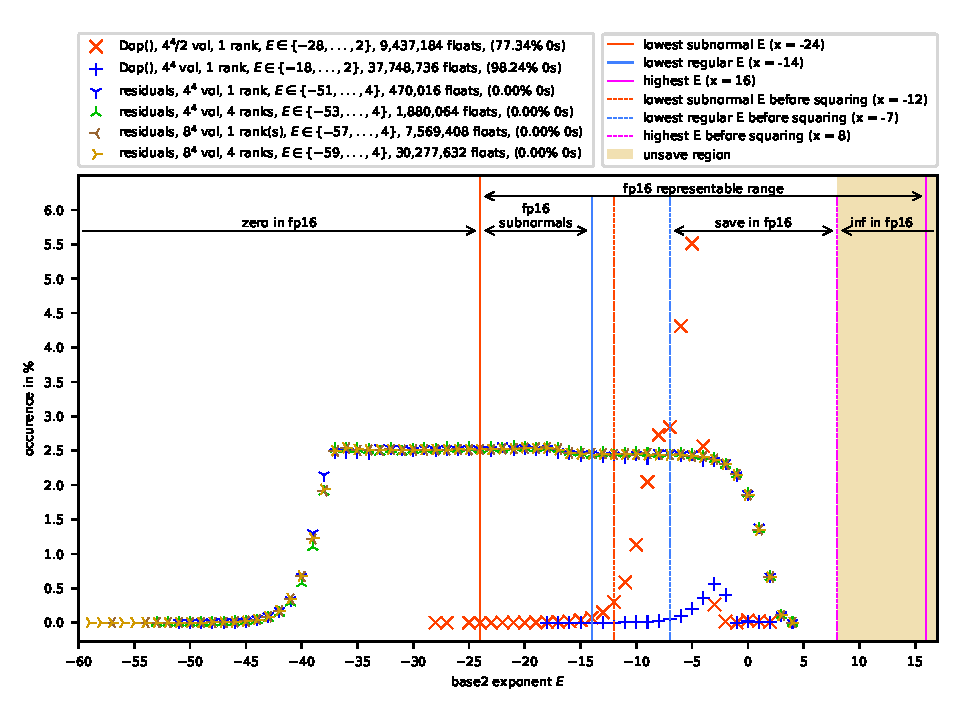
\includegraphics[width=1.0\textwidth]{plots/exponents_dirac}
    \caption{Exponent distribution of \gls{binary32} single precision floats in the residual vectors of all steps in a conjugate gradient run in openQxD as well as entries of the Dirac operator. 4 runs were made, with a lattice size of $4^4$ and $8^4$ on one single rank and $4$ ranks respectively. The number is normalised to $(-1)^s \cdot M \cdot 2^{E}$, where $M \in [1, 2)$.}
    \label{fig:exponents}
\end{figure}

\subsection{The conjugate gradient kernel}

The conjugate gradient kernel \code{cgne()} in \code{modules/linsolv/cgne.c} in \cite{openqxd} implements the algorithm, see Listing \ref{lst:cgne}.

\begin{figure} % wrap into a figure such that the whole snippet is on the same page
\begin{lstlisting}[
    language=C,
    firstnumber=429,
    label=lst:cgne,
    caption={The conjugate gradient kernel in \code{modules/linsolv/cgne.c} line \num{429}ff.}
]
double cgne(int vol,int icom,void (*Dop)(spinor *s,spinor *r),
            void (*Dop_dble)(spinor_dble *s,spinor_dble *r),
            spinor **ws,spinor_dble **wsd,int nmx,double res,
            spinor_dble *eta,spinor_dble *psi,int *status)
{
\end{lstlisting}
\end{figure} 

The function expects the Dirac matrix \code{Dop()} in \gls{binary32}, \code{Dop\_dble()} in \gls{binary64} format and the source vector \code{eta} ($\vec{b}$) in \gls{binary64} only. In the initialisation the starting vector \code{psi} ($\vec{x}_0$) is set to zero. The algorithm stops when the desired maximal relative residue \code{res} ($=\frac{\norm{\code{eta}-D^\dagger D \code{psi}}}{\norm{\code{eta}}}$) is reached, where \code{psi} is the calculated approximate solution of the Dirac equation $D^\dagger D \code{psi}=\code{eta}$ in \gls{binary64}. For this, the tolerance \code{tol} is calculated using $\code{tol} = \norm{\code{eta}} * \code{res}$. The parameter \code{nmx} is the maximal number of iterations that may be applied and \code{status} reports the total number of iterations that were required, or a negative value if the algorithm failed. \code{icom} is a control parameter and \code{ws} and \code{wsd} are wordspace allocations. The volume of the lattice should be given in \code{vol}.

Since the Dirac matrix is given in two precisions, the algorithm in the code bails out of the main conjugate gradient loop, when some particular conditions where met, see Listing \ref{lst:break}.

\begin{figure} % wrap into a figure such that the whole snippet is on the same page
\begin{lstlisting}[
    language=C,
    firstnumber=490,
    label=lst:break,
    caption={break condition in \code{modules/linsolv/cgne.c} line \num{490}ff, \code{rn} is the norm of the current residual, \code{xn} is the norm of the current solution vector, both in \gls{binary32}.}
]
if ((rn<=tol)||(rn<=(PRECISION_LIMIT*xn))||(ncg>=100)||
    ((*status)>=nmx))
   break;
\end{lstlisting}
\end{figure} 

This may happen in 4 cases:

\begin{enumerate}
  \item if the recusively calculated residual is below the tolerace,
  \item if the precision of \gls{binary32} is reached\footnotemark,
  \item after a hardcoded number of \num{100} steps,
  \item if the maximal number of steps is reached.
\end{enumerate}

\footnotetext{The constant \code{PRECISION\_LIMIT} is defined to be \code{100*MACHINE\_EPSILON}, where the \code{MACHINE\_EPSILON} is the difference between \num{1} and the lowest value above \num{1} depending on the datatype. In case of \gls{binary32} the \code{MACHINE\_EPSILON} takes a value of \num[round-mode = figures, round-precision = 8, scientific-notation = true]{1.1920928955078125e-07}.}

Point 2 is the most interesting condition, because lets imagine that this condition is met, but the algorithm does not break out of the main loop. Therefore the norm of the current residual compared to the norm of the current solution vector differ in their orders of magnitude by the precision limit of the datatype (\gls{binary32} in this case). This means that the solution vector $\vec{x_i}$ contains large numbers compared to the residual vector $\vec{r_i}$. Therefore the changing in residual from iteration to iteration is small compared to numbers in $\vec{x_i}$ as well. Since $\vec{r_i}$ contains small numbers, the amounts $\alpha_i$ are small as well. This causes $\vec{x_{i+1}} = \vec{x_i} + \alpha_i \vec{d_i}$ to not change anymore, because adding very large and very small numbers in floating point arithmetic will return the larger number unchanged if the two numbers differ in magnitude by the precision limit of the datatype. The algorithm stalls in that case and breaking out of the main loop is the emergency brake.

So when one of the above conditions are met, the algorithm performs a \df{reset step}. A reset step consists of calculating the residual not in the recursive way, instead calculating it in it's definition $\vec{r_i} = \vec{b} - A \vec{x_i}$ in double precision. This involves \num{2} invocations of each \code{Dop\_dble()} as well as \code{Dop()} which is very expensive. The algorithm is resetting in the sense that the solution vector is set back to $\vec{x_i} = 0$, but before resetting, the solution vector in \gls{binary32} is added to the real solution vector \code{psi} in \gls{binary64} which was initialied to zero at the start of the algorithm as well. It looks like a restart of the whole calculation, but the direction for the next iteration $\vec{d_i} = \vec{r_i}$ is set to the just calculated, very accurate residual. Therefore the the algorithm now continues in a new direction $A$-orthogonal to all previous directions and progression is kept. The step is meant to remove the accumulated roundoff errors due to the recursive calcuation of the residuals and directions. The first step following a reset step is a step in the direction of steepest descent just like the very first step of the algorithm. The less precise the datatype, the more reset steps need to be taken, because the precision limit is reached earlier.

\subsection{Simulating other datatypes}

Some operations such as norms and scalar products are memory-bandwidth-bound, which means the on-chip memory bandwidth determines how much time is spent computing the output. Storing input data in a format with lower bit-length reduces the amount of data to be transferred, thus improving the speed of calculation.

The complete conjugate gradient kernel was simulated in different datatypes, floats as well as posits. In order to produce the plots, the dirac matrix \code{Dop\_dble()} and the source vector $\code{eta}$ were extracted in \gls{binary64} format from the original code running a simulation of a $4^4$ lattice, \acrfull{sf} boundary conditions (\code{type 1}), no C* boundary conditions (\code{cstar 0}) and $1$ rank. The first \num{2000} trajectories were considered of thermalization. The matrix was extracted in trajectory \num{2001}. A python script mimicking the exact behavior of the \code{cgne()} kernel from the source code\footnotemark, was implemented to cope with arbitrary datatypes. The simulated datatypes were \gls{binary64}, \gls{binary32}, \gls{tensorfloat32}, \gls{binary16}, \gls{bfloat16}, \gls{posit32}, \gls{posit16}, and \gls{posit8}. The Dirac matrix had approximately \num{2}\% non-zero value. The results are plotted in figures \ref{fig:cgne:naive}, \ref{fig:cgne:quire}, \ref{fig:cgne:col64} and \ref{fig:cgne:res12}.

\footnotetext{See line 429ff in \code{modules/linsolv/cgne.c} in \cite{openqxd}.}

\begin{comment}
\begin{figure}
    \centering
    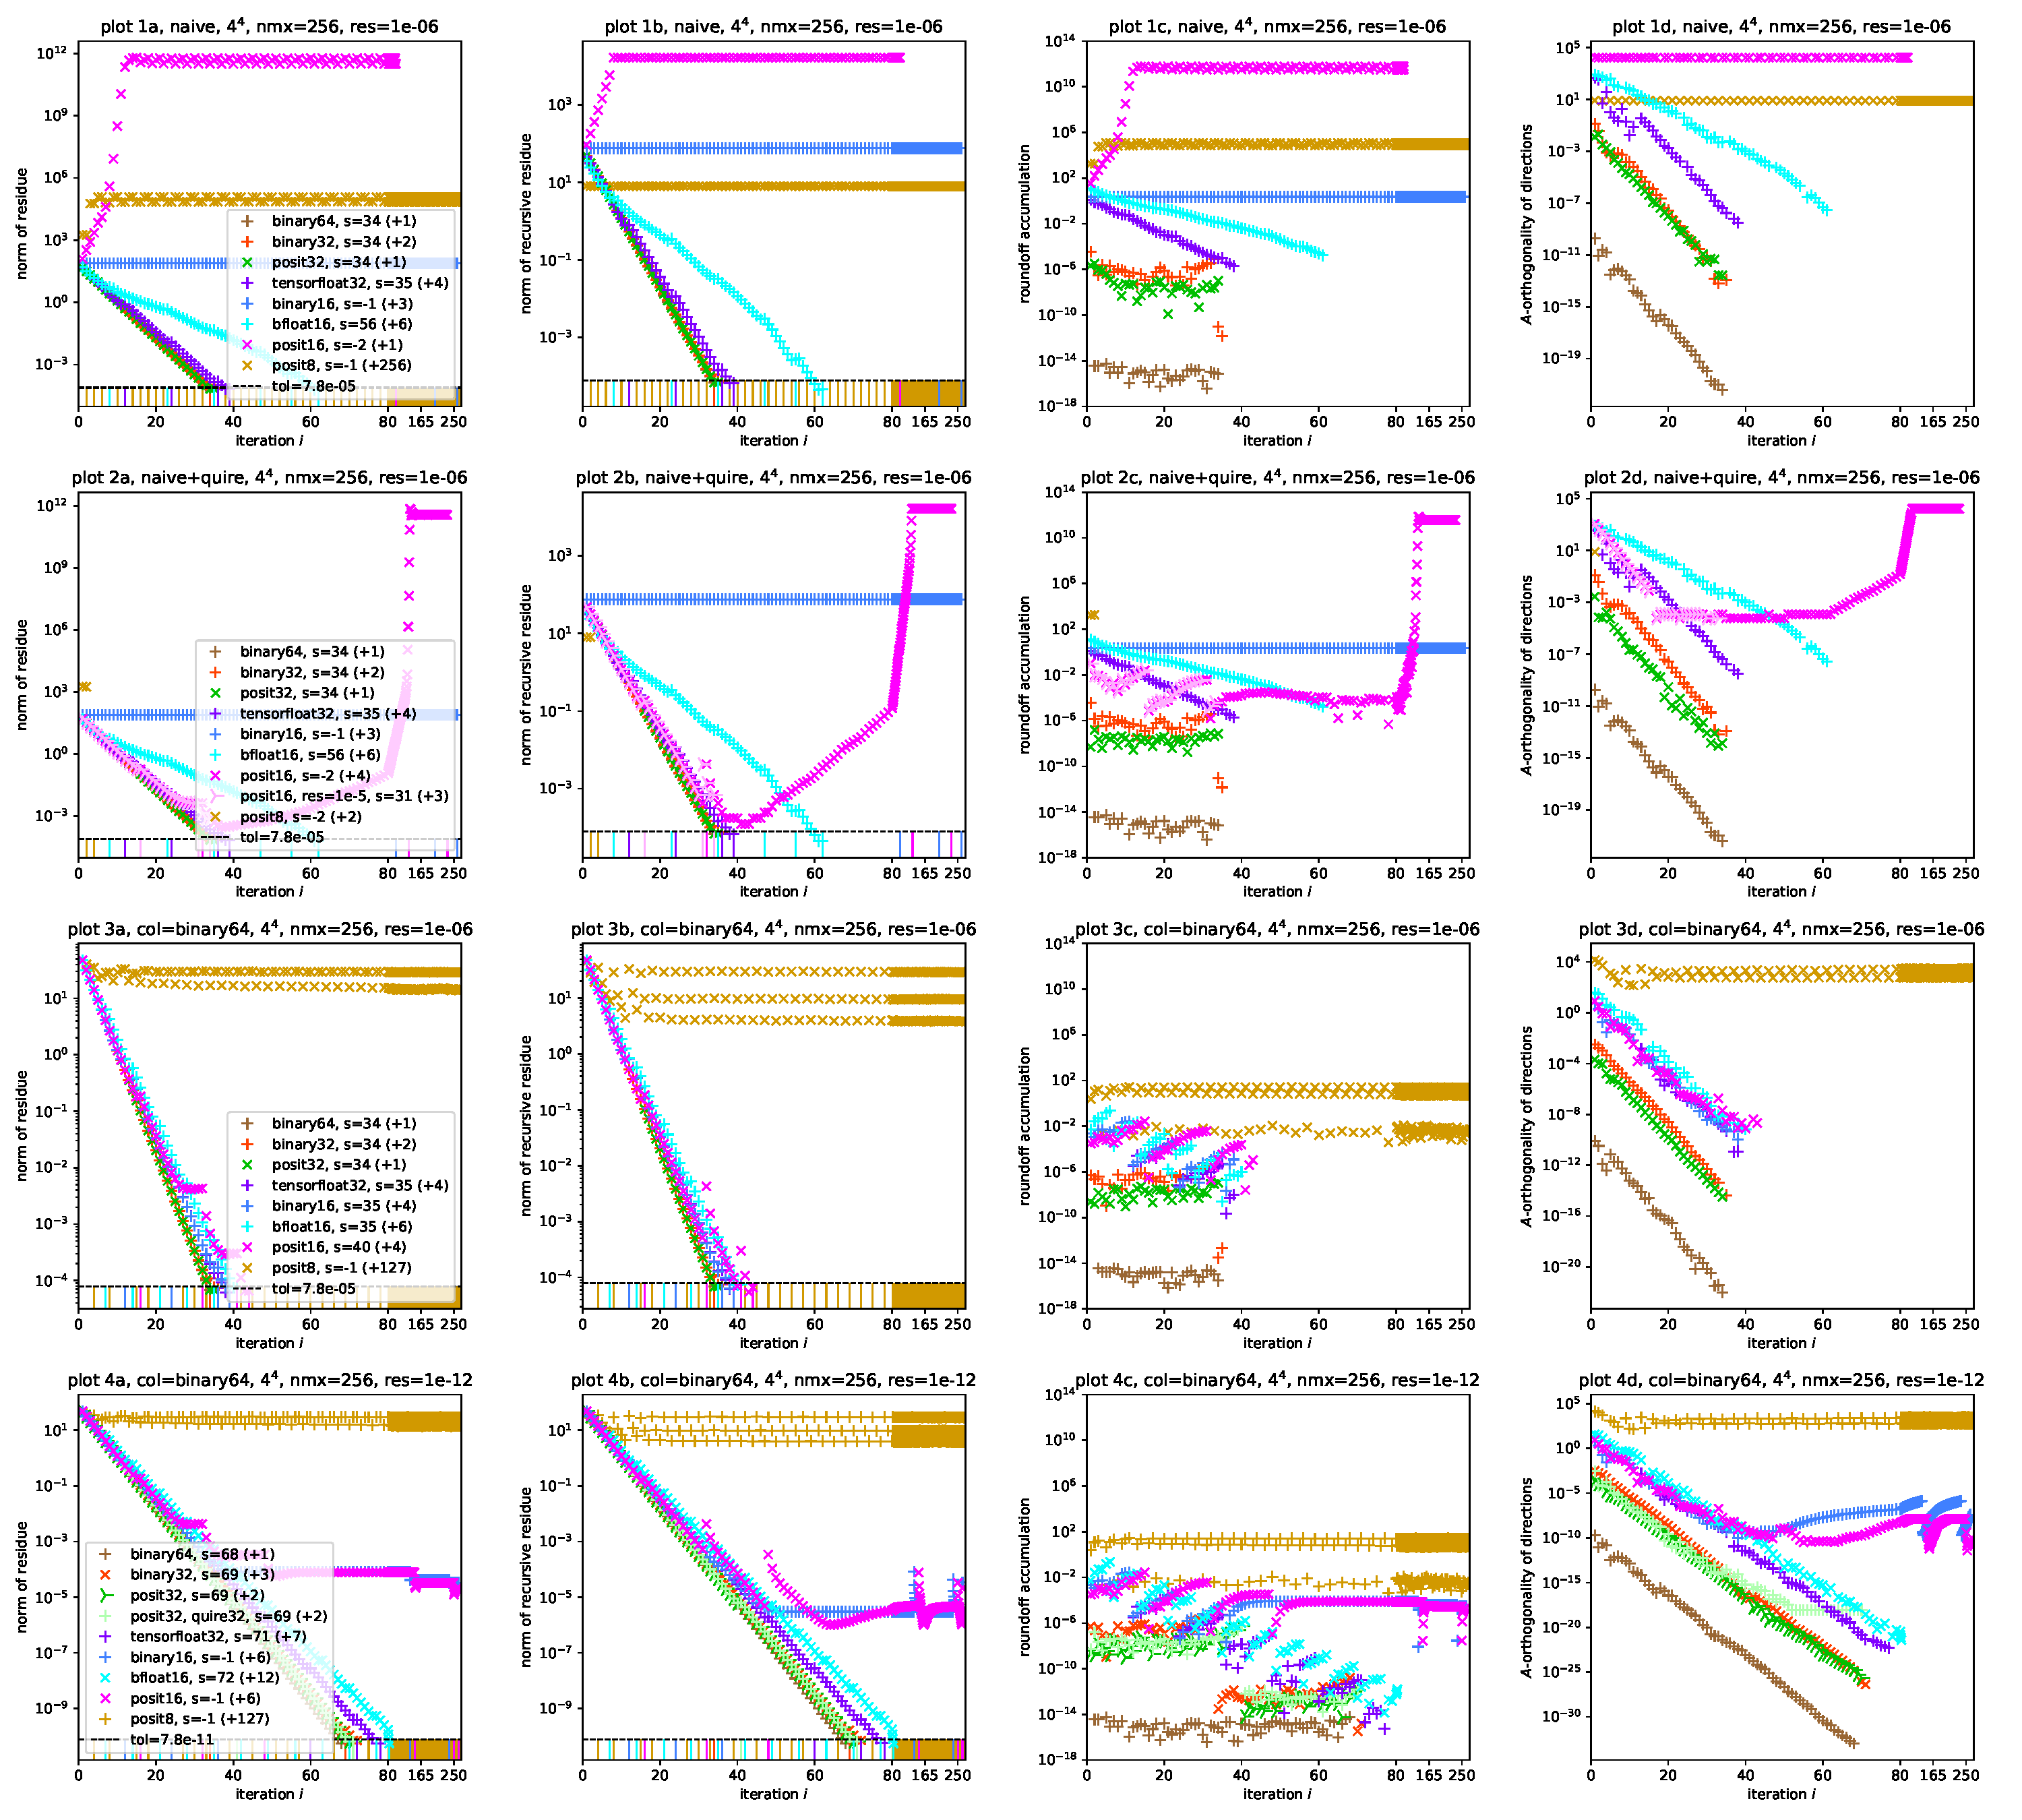
\includegraphics[width=1.0\textwidth]{plots/cgne}
    \caption{Convergence analysis of a conjugate gradient run, where \gls{binary32} was replaced by one of the simulated datatypes. The legend for every row is equal, displayed only in the first plot of the row. The number \code{s} describes the number of normal steps needed (the value of \code{status}), whereas the numbers in the brackets indicates the number of reset steps. All reset steps are indicated by ticks at the dashed black tolerance line. The iterations will always go up to \code{nmx=256}, but the range \num{80}-\num{256} is compressed since the most interesting behavior happens before step \num{80} for most of the simulated datatypes. The \textit{first row} shows a naive replacement of the \gls{binary32} datatype with the simulated one. This means that every single variable containing a \gls{binary32} was replaced with a variable of the simulated datatype. Plot \textit{1a} shows the exact residue \eqref{eq:residual_exact} in every iteration calculated using the Dirac matrix and the source vector both in \gls{binary64}, whereas plot \textit{1b} shows the norm of the recursively calculated residue \eqref{eq:residual_recursive} (casted after the calculation from the simulated datatype to \gls{binary64}). The relative residue suffers roundoff accumulation because of the recusive calculation; this is the differnce between plots \textit{1a} and \textit{1b}, which is plotted in plot \textit{1c}. Plot \textit{1d} shows the $A$-orthogonality of the current direction to the last direction, namely the value of $\vec{p}_{i}^\dagger A \vec{p}_{i+1}$. In the \textit{second row}, the posits were utilizing \glspl{quire} as their collective variables, the remaining setup was the same as for the first row. The \textit{third row} introduces a slightly smarter replacement. All collective variables such as norms where calculated in \gls{binary64}, such that a datatype with a small number range such as \gls{binary16} may not over- or underflow when calculating the norm of a vector full of said datatype. This replacement resembles the \gls{quire} for posits. Using this replacement, even heavily reduced datatypes like \gls{binary16} and \gls{posit16} converged and threw a result of equal quality as the one simulated with \gls{binary64}. The configuration in the \textit{fourth row} is equal to the third row, besides the value of \code{res} - the desired relative residue of the calculated solution - is set to $10^{-12}$ instead of $10^{-6}$. Only the 32- and 64-bit number formats converged and gave a meaningful result. Notice that $10^{-12}$ is outside the representable number range of \gls{binary16}, \gls{posit16} and \gls{posit8}.}
    \label{fig:cgne}
\end{figure}
\end{comment}

\begin{figure}
    %\centering
    \makebox[\textwidth][c]{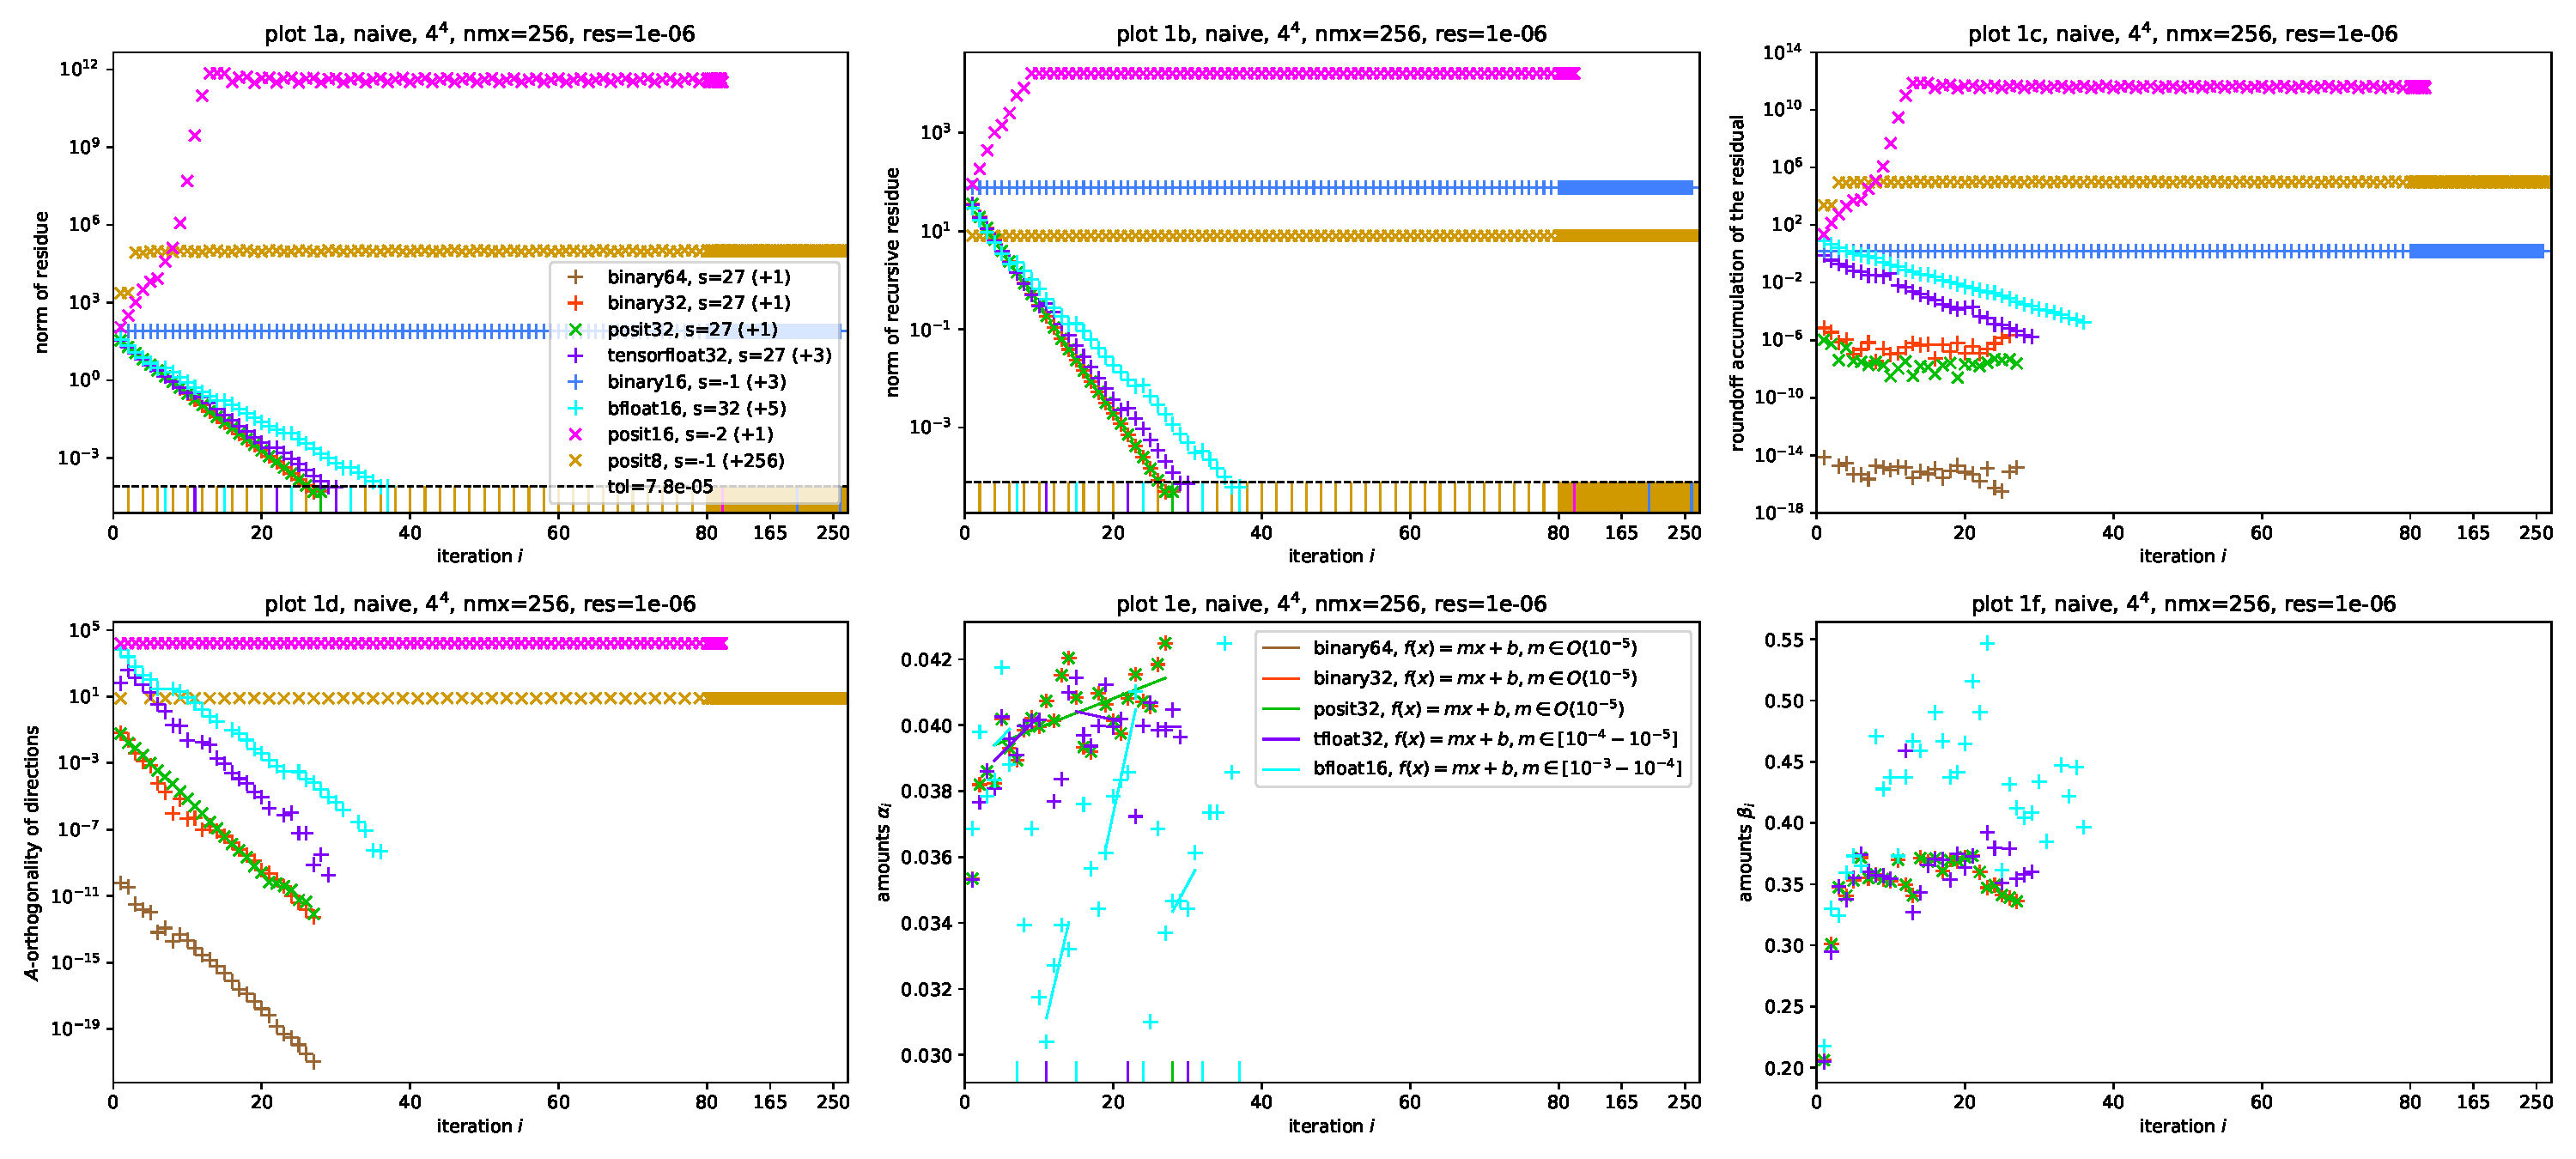
\includegraphics[width=1.0\linewidth]{plots/cgne_new0}}
    %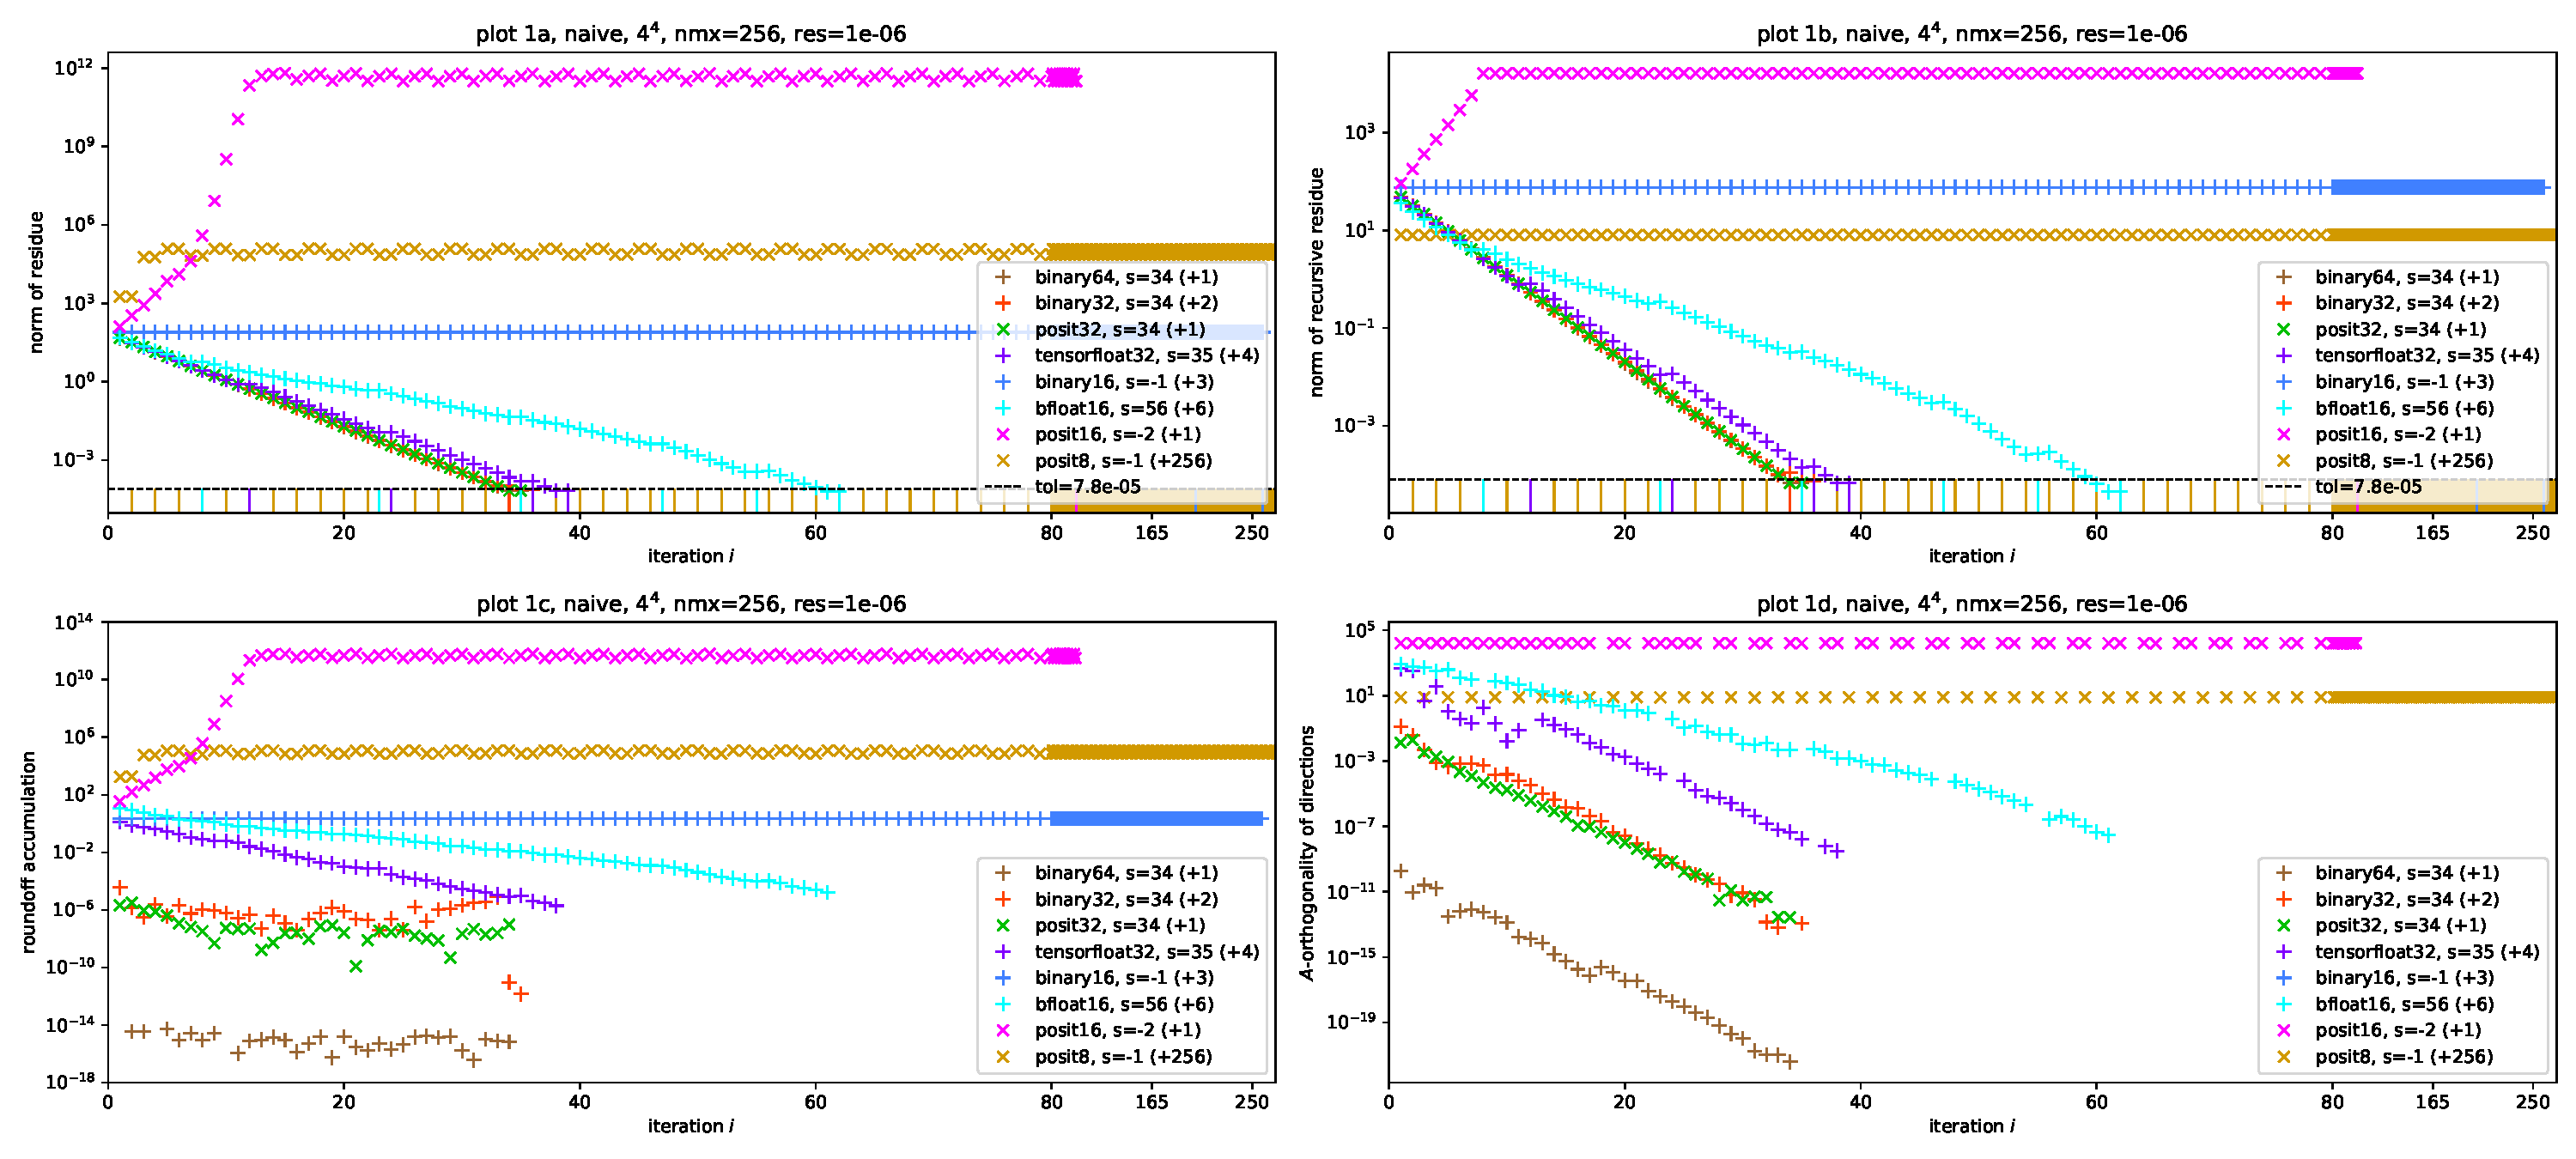
\includegraphics[width=1.0\textwidth]{plots/cgne0}
    \caption{Convergence analysis of a conjugate gradient run, where \gls{binary32} was replaced by one of the simulated datatypes. The number \code{s} describes the number of normal steps needed (the value of \code{status}), whereas the numbers in the brackets indicate the number of reset steps. All reset steps are indicated by ticks at the dashed black line denoting the tolerance limit. The iterations will always go up to \code{nmx=256}, but the range \num{80}-\num{256} is compressed since the most interesting behavior happens before step \num{80} for most of the simulated datatypes. The 6 plots show the naive replacement of the \gls{binary32} datatype with the simulated one. This means that every single variable containing a \gls{binary32} was replaced with a variable of the simulated datatype. Plot \textit{1a} shows the exact residue \eqref{eq:residual_exact} calculated in every iteration using the Dirac matrix and the source vector both in \gls{binary64}, whereas plot \textit{1b} shows the norm of the recursively calculated residue \eqref{eq:residual_recursive} (casted from the simulated datatype to \gls{binary64}). The relative residue suffers roundoff accumulation because of the recusive calculation; this is the differnce between plots \textit{1a} and \textit{1b}, which is plotted in plot \textit{1c}. Plot \textit{1d} shows the $A$-orthogonality of the current direction to the last direction, namely the value of $\vec{p}_{i}^\dagger A \vec{p}_{i+1}$. The last 2 plots, \textit{1e} and \textit{1f}, show the values of the amounts $\alpha_i$ and $\beta_i$ (see equations \eqref{eq:alphai} and \eqref{eq:betai}) in every iteration, but only of the datatypes that converged (\code{status>0}). The lines in plot \textit{1e} are linearly fitted to the data points ($f(x) = m x + b$). The number range of the slope $m$ is given in the plot legend.}
    \label{fig:cgne:naive}
\end{figure}

\begin{figure}
    \centering
    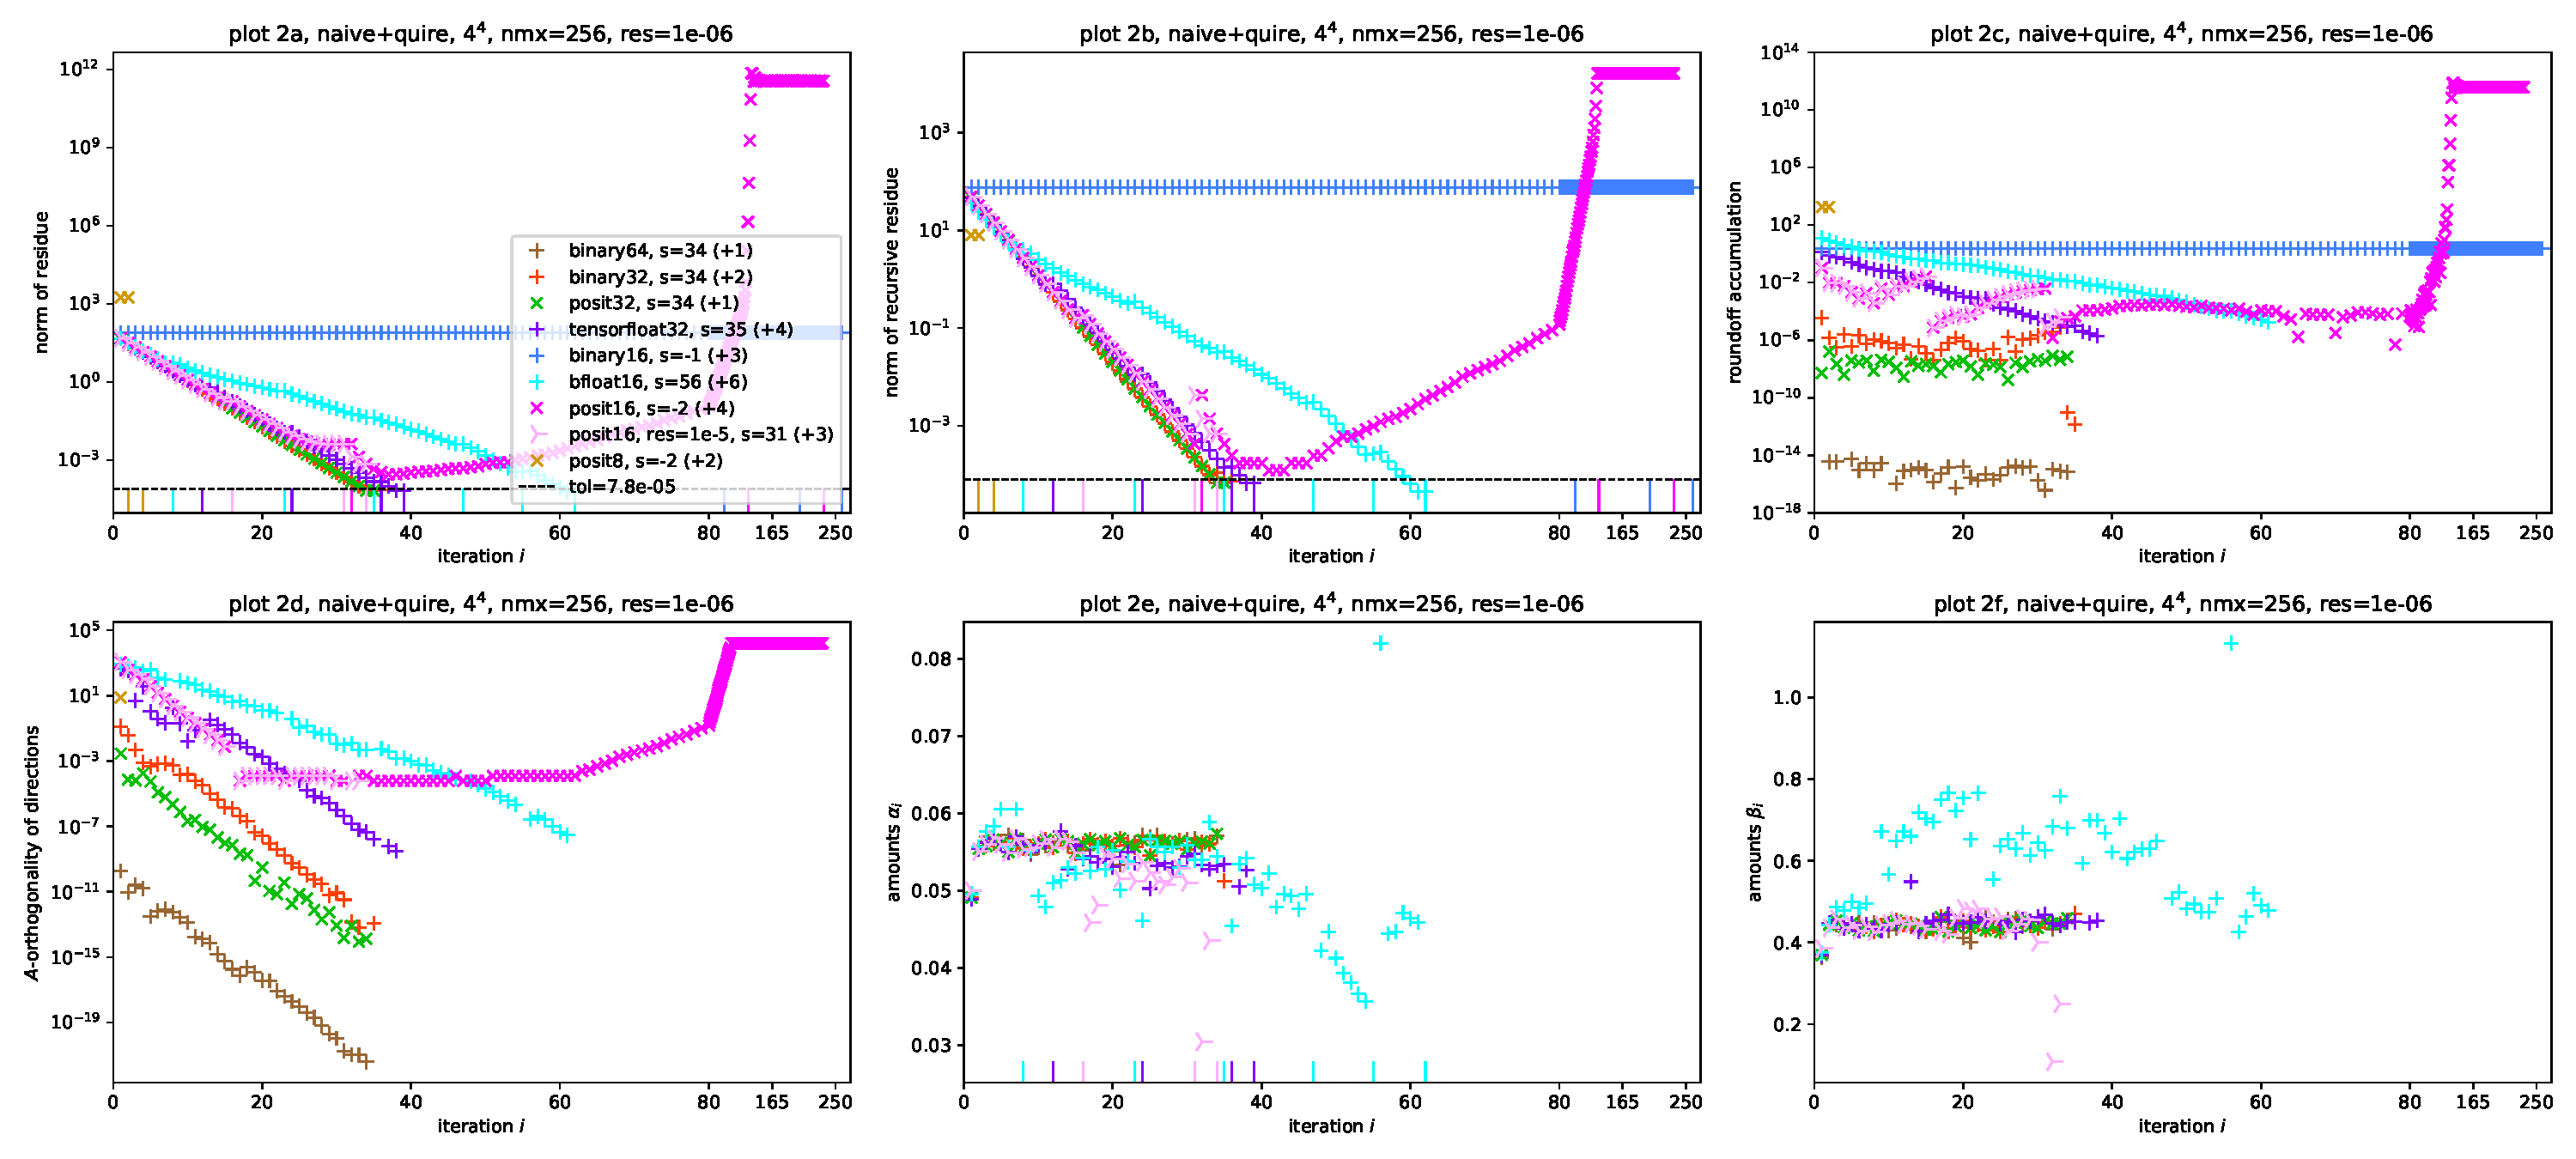
\includegraphics[width=1.0\textwidth]{plots/cgne_new1}
    \caption{In these plots, the posits were utilizing \glspl{quire} as their collective variables, the remaining setup was the same as for firgure \ref{fig:cgne:naive}, therefore the floating point datatypes show exactly the same values, only posits changed their behavior.}
    \label{fig:cgne:quire}
\end{figure}

\begin{figure}
    \centering
    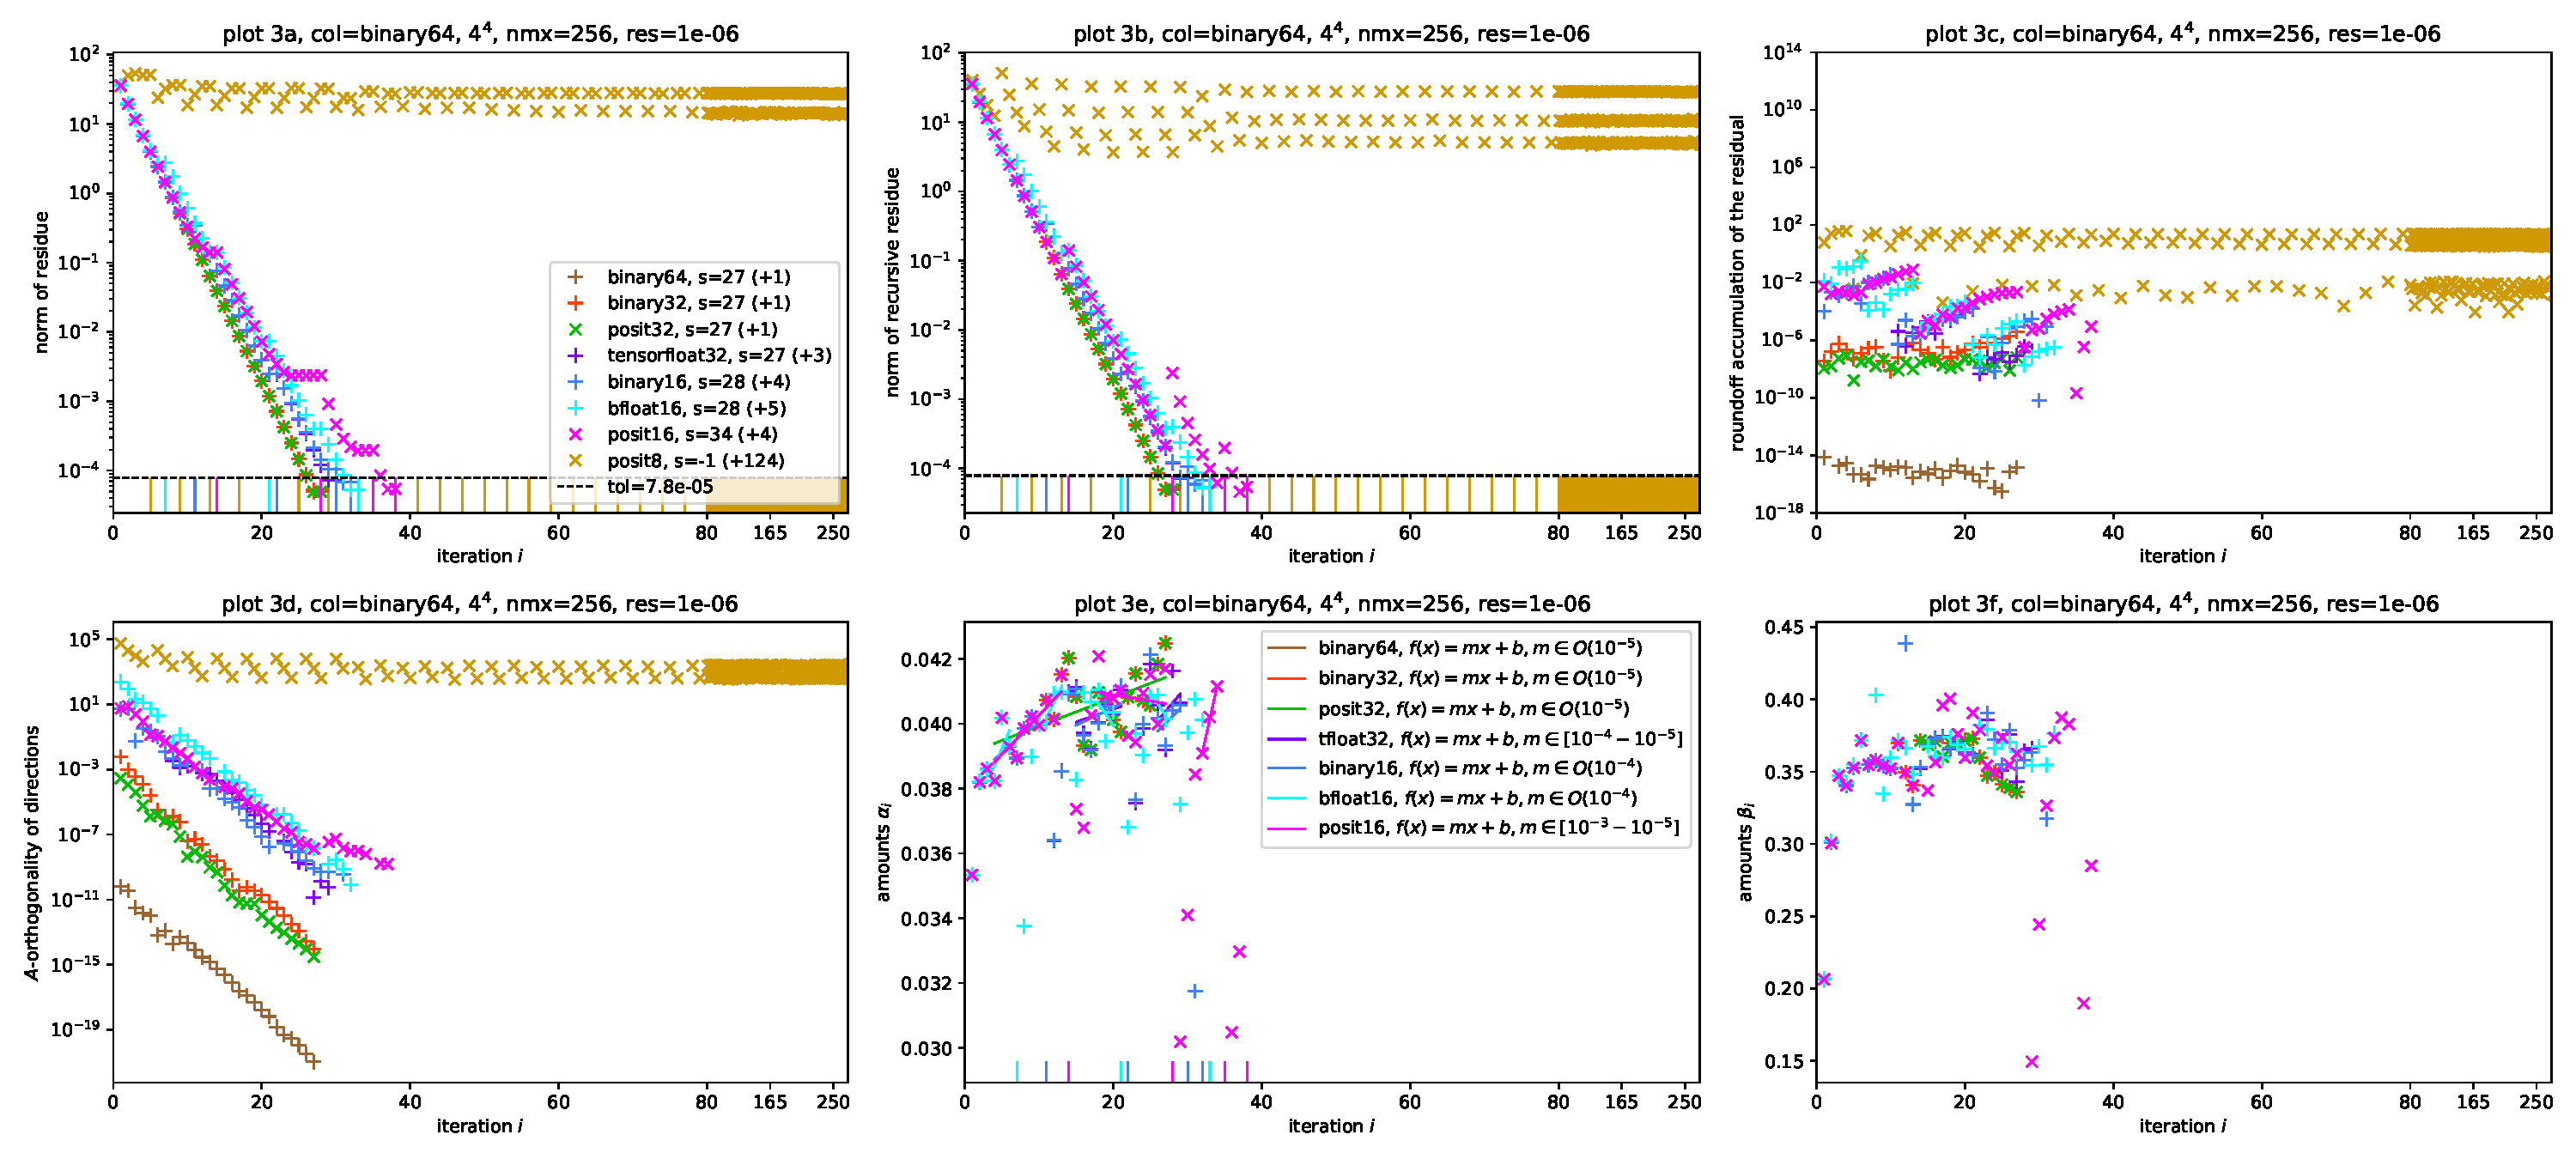
\includegraphics[width=1.0\textwidth]{plots/cgne_new2}
    \caption{The 6 plots introduce a slightly smarter replacement. All collective variables such as norms where calculated in \gls{binary64}, such that a datatype with a small number range such as \gls{binary16} may not over- or underflow when calculating the norm of a vector full of said datatype. This replacement resembles the \gls{quire} for posits. Using this replacement, even heavily reduced datatypes like \gls{binary16} and \gls{posit16} converged and threw a result of equal quality as the one simulated with \gls{binary64}.}
    \label{fig:cgne:col64}
\end{figure}


\begin{figure}
    \centering
    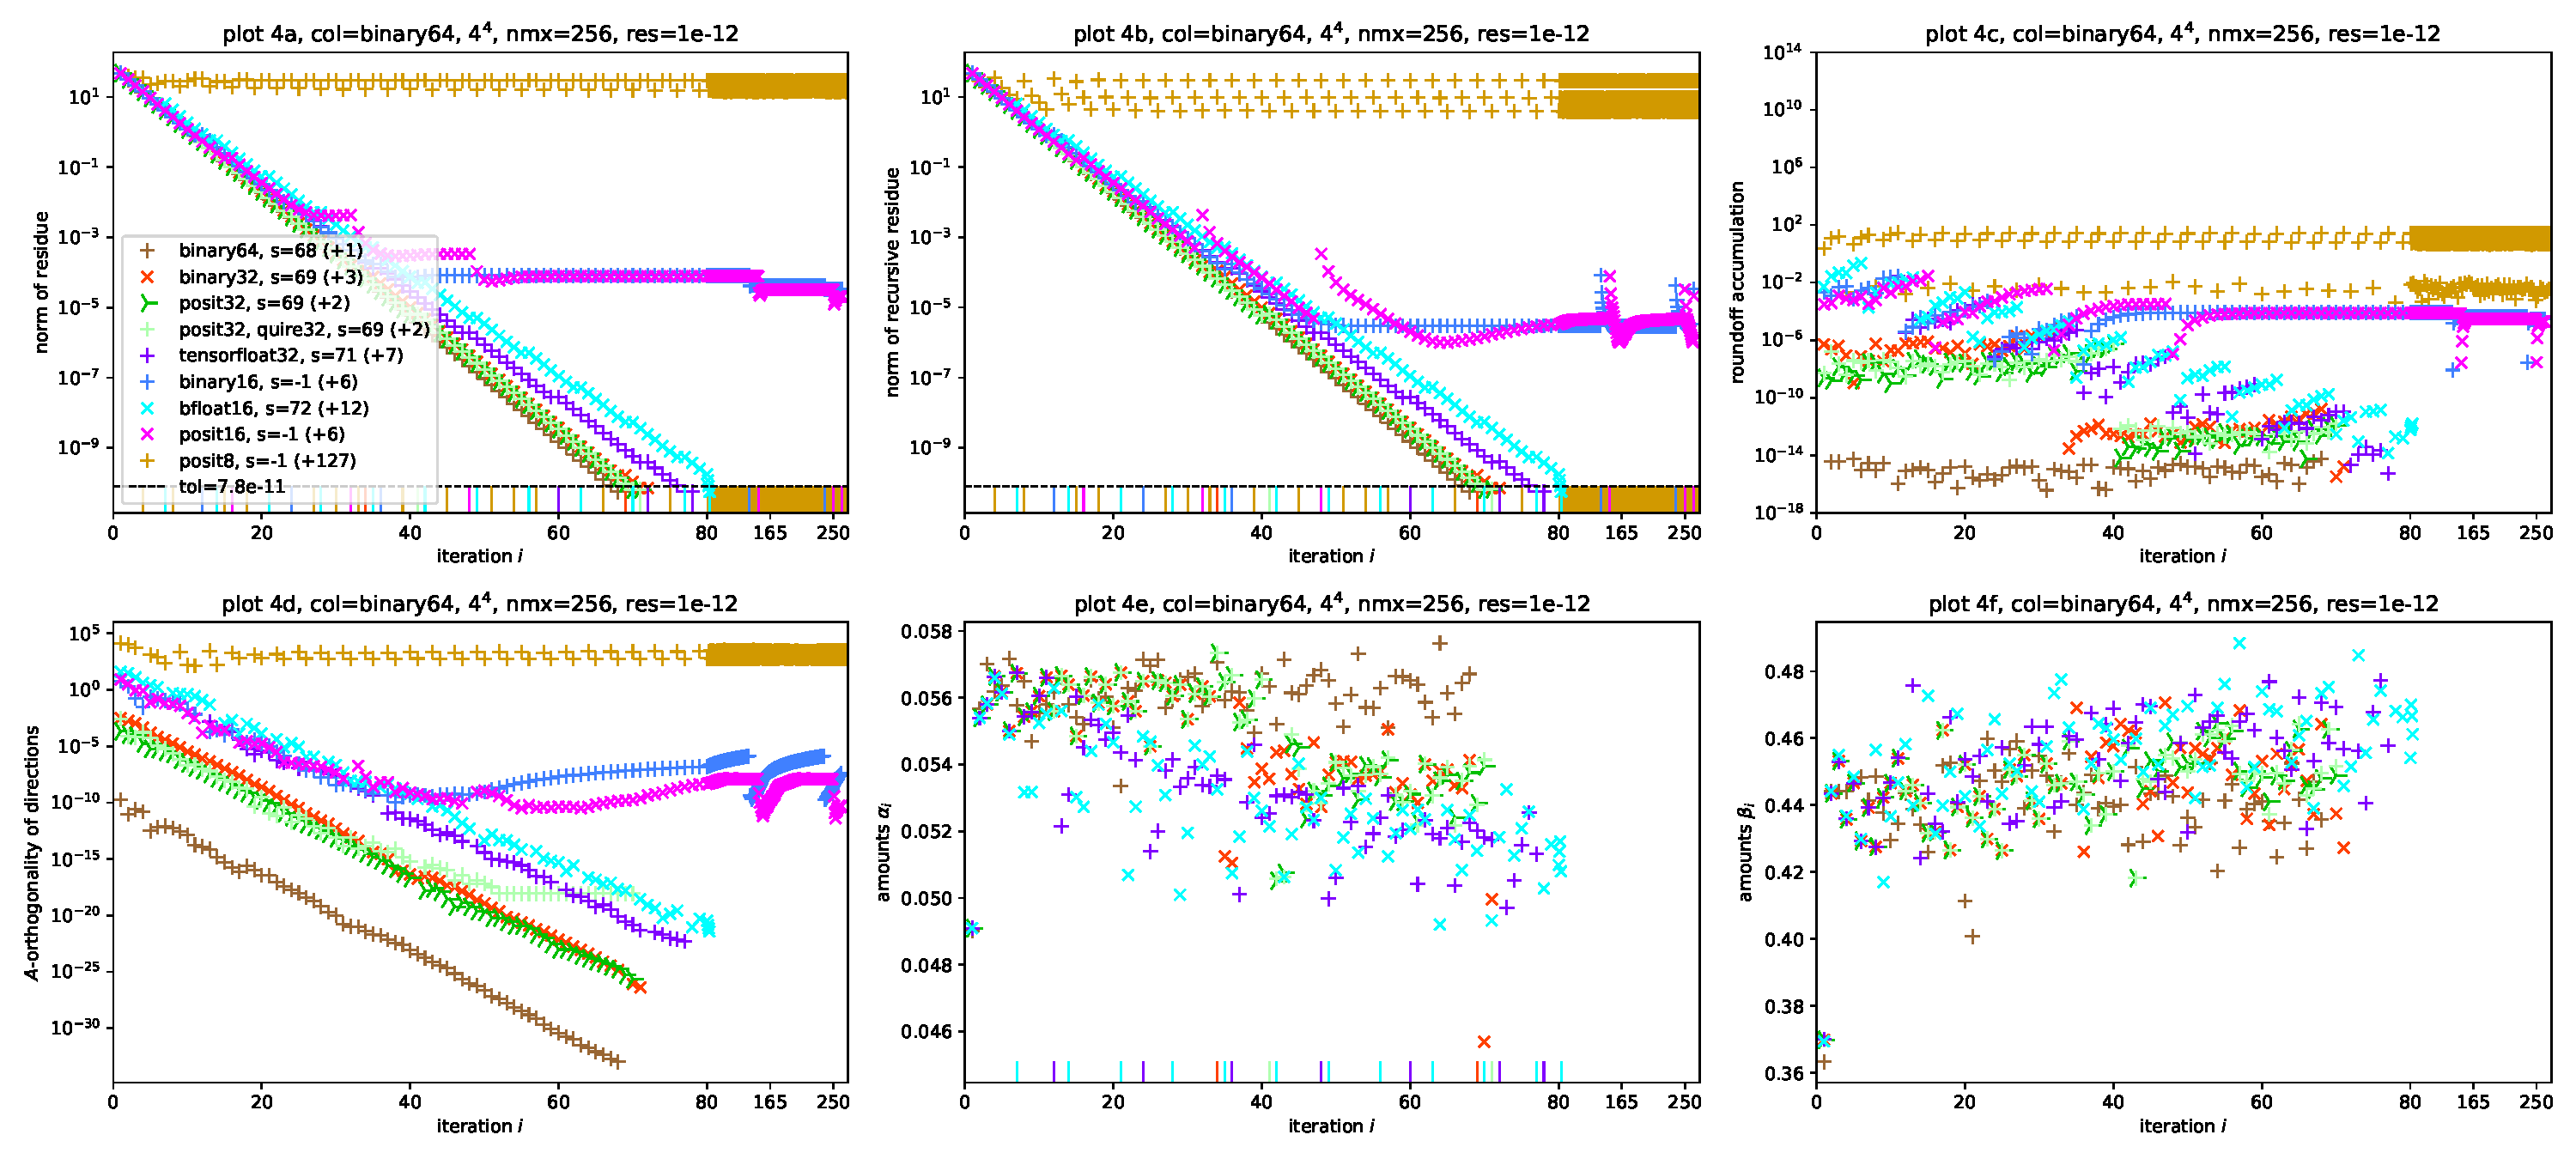
\includegraphics[width=1.0\textwidth]{plots/cgne_new3}
    \caption{The configuration in this series of plots is equal to Figure \ref{fig:cgne:col64}, besides the value of \code{res} - the desired relative residue of the calculated solution - is set to $10^{-12}$ instead of $10^{-6}$. Notice that $10^{-12}$ is outside the representable number range of the datatypes that did not converge; \gls{binary16}, \gls{posit16} and \gls{posit8}.}
    \label{fig:cgne:res12}
\end{figure}

\subsubsection{Discussion of figures \ref{fig:cgne:naive} - \ref{fig:cgne:res12}}

Figures \ref{fig:cgne:naive}, \ref{fig:cgne:quire}, \ref{fig:cgne:col64} and \ref{fig:cgne:res12} contain all relevant data. It is expected in general that the plots show datatypes of the same bit-length in clusters and exhibit a hierarchy in precision and exponent range; more precision and larger exponent range should end up in faster convergence. Thus we expect the following hierarchy (where smaller means convergence in fewer steps)

\begin{align}
    \textcolor{cbrown}{\text{binary64}} < \textcolor{cgreen}{\text{posit32}} \leq \textcolor{cred}{\text{binary32}} \leq \textcolor{cpurple}{\text{tensorfloat32}} \leq \textcolor{cturquois}{\text{(1)}} \leq \textcolor{cpink}{\text{posit16}} \leq \textcolor{cblue}{\text{binary16}} \leq \textcolor{cturquois}{\text{(2)}} < \textcolor{cyellow}{\text{posit8}}, \label{eq:hierarchy}
\end{align}

where \textcolor{cturquois}{\text{bfloat16}} could be either at position \textcolor{cturquois}{\text{(1)}} or \textcolor{cturquois}{\text{(2)}}, depending on what is more important; precision or number range.

In Figure \ref{fig:cgne:naive} where the datatype is naively replaced by the simulated datatype, it can be concluded that only datatypes with large enough number ranges converged. \gls{binary64}, \gls{binary32} and \gls{posit32} converged each after \code{status=27} steps with one reset step. The less precise \gls{tensorfloat32} took \code{status=27} ($+3$) and the even less precise \gls{bfloat16} needed \code{status=32} ($+5$) steps. Such a hierarchical result was expected since they have the same exponent range and thus approximately the same number range, but differ only in precision (see Table \ref{tab:formats}). Notice that the less precise the datatype, the more reset steps are needed. This happens because the precision limit of the simulated datatype is reached faster, if the datatype has less precision.

The roundoff accumulation error of \gls{posit32} is slightly better than the one of \gls{binary32}, although defeated by $8$ orders of magnitude of \gls{binary64} because of its much more precision. It is notable to remark that the roundoff accumulation does not increase substantially from step to step, what would be expected from a recursive calculation. The reason for the small difference between \gls{binary32} and \gls{posit32} could be that the involved real numbers are closer to representable numbers in \gls{posit32} than in \gls{binary32}. Posits have a larger number density around \num{1} compared to floats of the same bit-length, and therefore more precision in that regime (see Figure \ref{fig:number_line} for the example of \gls{binary16} versus \gls{posit16}). Posits also have more numbers, because they have no \acrshortpl{nan}. Roundoff accumulation is specially dependent on the precision of the datatype, which makes sense; the lower the precision, the higher the roundoff accumulation. The difference in $A$-orthogonality is neglectible for \gls{posit32} compared to \gls{binary32}, but again clearly surpassed by \gls{binary64}.

\gls{binary16} did not converge (\code{status=-1}) after the maximal number of \code{nmx=256} steps. Its footprint is absent in plot \textit{1d}, because it consisted only of \acrshortpl{nan} and infinities, causing $\alpha_i = 0$ and $\beta_i = 1$. This implied that $\vec{r}_i = \vec{r}_{i+1}$ and $\vec{p}_{i+1} = \vec{r}_{i+1}$ and therfore $\vec{x}_{i+1} = \vec{x}_{i}$ and the algorithm stalled. This explains the residues not changing in plots \textit{1a} and \textit{1b}. The reason for the first infinity was an overflow when calculating the norm of $\vec{b}$ in the very first iteration. This suggests that the limited number range of \gls{binary16} might not be enough (at least for a naive replacement), comparing to \gls{bfloat16} with the same bit-length, but larger number range that was able to converge, although very slowly.

The behavior of \gls{posit8} is very similar to \gls{binary16}, but without the overflow, because posit do not overflow by definition. Instead the biggest representable number is returned or in case of an underflow the smallest representable number is returned \cite{posit2018standard}. The algorithm stalled at a value of the norm of the recusive residual of $\norm{\vec{r}_i} = 8$. The biggest \num{8}-bit posit number with exponent bits $es=0$ is $2^6 = 64$, so the norm squared cannot be bigger than $64$ and the norm itself cannot be bigger than $8 = \sqrt{64}$ (see plot \textit{1b}). This happend in the first step, whereas the actual residual in \gls{binary64} was $\backsim 10^3$. The amounts $|\alpha_i| \ll 1$ in iterative steps are therfore very small causing $\vec{x}_{i+1} \approx \vec{x}_i$. Significant changes in $\vec{x}_i$ will not happen and convergence is unlikely. Also notice that \gls{posit8} had \num{256} reset steps, which means that after every step there was a reset step. The steps where caused by the very high precision limit of \gls{posit8}. The value of \code{PRECISION\_LIMIT} is $100*\code{MACHINE\_EPSILON}$, which has a value of \num{3.125} for \gls{posit8}.

The story of \gls{posit16} is very similar, just that the maximal representable value with $es=1$ is \num{268435456} and the square root of this is \num{16384} which is reached after $8$ steps (see plot \textit{1b}). The actual residual in the $8$-th step was $\backsim 10^7$, the algorithm diverged and then stalled. Iterative steps are therfore mostly too small and convergence is unlikely.

We observe that number range is more important than precision, when naively replacing the datatype, but the higher the precision, the faster the convergence and the less reset steps needed.

In Figure \ref{fig:cgne:quire} the replacement utilised the possibility to use \glspl{quire} for the posit runs. Therefore, the numbers for the float datatypes are exactly equal to the ones in Figure \ref{fig:cgne:naive}, because floats have no such feature. They are not discussed again.

Comparing plots \textit{1c} and \textit{2c} and looking at \gls{posit32}, one can see that the roundoff accumulation in the residual due to its recursive calculation is slightly better than without using the \gls{quire}. This makes sense, because \glspl{quire} introduce deferred rounding. This is exploited specially in the calculation of norms and matrix-vector products. It also results in a somewhat better maintaining of $A$-orthogonality for the direction vectors.

However, the data points of \gls{posit16} bear little resemblance to its previous or later runs. It comes much closer to the target residual tolerance than in the last simulation, but it is still not reached. The tolerance is within the number range of \gls{posit16}, even so it did not converge. The reason for this is that the smallest representable number in \gls{posit16} is $2^{-28}$. The \gls{quire} for \gls{posit16} has the same number range, despite the \num{128} bits in length. Every norm squared of a non-zero vector must be larger to equal to this number, because posit do not underflow. Therefore the norm is always larger or equal to $\sqrt{2^{-28}} = 2^{-14} \approx 6.1 \cdot 10^{-5}$. The tolerance of $7.8 \cdot 10^{-5}$ - even though larger than that number - is perhaps still too close. Comparing the \textcolor{clightpink}{lightpink} values, that are \gls{posit16} as well, but the relative residual \code{res} is set to $10^{-5}$ instead (the tolerance being one order of magnitude larger), they converged after only \code{status=24} steps. This suggests that the reason for the strange behavior lies in the relative residual that was chosen too close to the lowest number above zero of the number regime.

Using the same arguments and analysis, \gls{posit8} had no chance to give a meaningful result.

In Figure \ref{fig:cgne:col64}, a smarter replacement was done. All variables that have a colletive role suffer from overflow. For example the norm of a vector $\vec{v} \in \mathbb{R}^n$ is 

\begin{align*}
    \norm{\vec{v}} = \sqrt{ \sum_{i=1}^{n} v_i^2 }.
\end{align*}

The number below the square root may be much bigger before squaring than after. If we calculate the norm in \gls{posit8}, the result will be $\norm{\vec{y}} \leq 8$. More importantly, when using a datatype that overflows such as \gls{binary16}, the value after squaring might be perfectly fine, but the value under the square root could be outside the range of representable numbers, $\sqrt{\infty} = \infty$ and $\sqrt{0} = 0$. This is cured if the collective variable is of a datatype with larger number range than the underlying datatype that is summed over. In Figure \ref{fig:cgne:col64} all collective variables were of type \gls{binary64}.

The data of \gls{binary64} exhibits no significant alterations. Again comparing \gls{binary32} and \gls{posit32} with their previous data points, we see that the roundoff accumulation of \gls{binary32} is a little better and \gls{posit32} is approximately the same as with the \gls{quire}, suggesting that when using posits utilizing the \gls{quire} is probably sufficient.

Looking at \gls{tensorfloat32}, it has the same exponent range as \gls{binary32}, but less precision and it has the same number of mantissa bits as \gls{binary16}, but at a higher exponent range. Compared to \gls{binary16}, both datatypes have the same amount of numbers to be distributed in their respective number range. It is expected to perform worse or equal to \gls{binary32}, but better or equal to \gls{binary16} and \gls{bfloat16}. Therefore it's expected to converge in $27 \le \code{status} \le 28$ steps, see equation \eqref{eq:hierarchy}. This is indeed the case with \code{status=27} steps. We see that the larger number range compared to \gls{binary16} has little to do with speed of convergence. This is because the number regime is within the \gls{binary16} regime, except for collective variables. This explans as well why \gls{tensorfloat32} performed precisely as in the naive replacement, Figure \ref{fig:cgne:naive}, but the roundoff accumulation is better because of the more precise collective variables.

The \gls{bfloat16} with even less precision but comparable number range of \gls{tensorfloat32} converged in \code{status=28} steps as well, but needed two more reset steps, tightening the previous conclusion about speed of convergence.

The most interesting data points are the ones of \gls{binary16} and \gls{posit16} that both were able to converge in \code{status=28} and \code{status=34} steps respectively. They performed quite similar, even though it would be expected that \gls{posit16} would perform a slightly better because of the bigger number range and bigger number density in relevant number regimes (see Figure \ref{fig:number_line}). In plot \textit{3c} the increase of roundoff accumulation can be observed for \gls{binary16} and \gls{posit16} in steps where the real residue changes (where the algorithm makes progress, see for example: steps \num{1} to \num{10}). Notice that, when the real residue stalls and the recusive residue still (wrongly) decreases, the roundoff accumulation will saturate until the order of magnitude of the two numbers becomes too large such that their difference is dominated by the larger number. This can the seen in the data points of \gls{posit16} in plot \textit{3a}. It suggests that the precision limit was chosen too low for the datatype. Notice that the precision limit is defined to be \num{100} times the \code{MACHINE\_EPSILON} of the datatype. The \code{MACHINE\_EPSILON} for the posit datatypes is quite misleading, because it gives us (by definition) the precision of numbers around \num{1}. This is the regime where posits are most precise, their precision falling off very rapidly when leaving it. Thus for \gls{posit16} in the regime $10^{-1}$ the \code{MACHINE\_EPSILON} is correct (seen at iteration \num{14}), whereas in the regime $10^{-3}$ it is chosen to small and we can see a staircase-shape around the reset steps at iterations \num{28} and \num{35}. Such a stalling of the real residue should be avoided at any cost, because the algorithm stalls as well in that case. The \code{MACHINE\_EPSILON} is defined to be the difference between \num{1} and the lowest number above \num{1}. For floats this definition makes more sense, because their precision does not fall off that fast, but for posits which are most presice around \num{1} this gives a too precise value, not refecting the real precision of posits in their whole number range correctly. Instead, the machine epsilon should be a function of the number regime, increasing when going far away from \num{1}. This is the reason for the staircase-shaped curve of \gls{posit16} in plot \textit{3a}. The phenomenon is even more prominent for \gls{posit16} in plot \textit{4a} of Figure \ref{fig:cgne:res12}. The \gls{posit32} does not have this problem, because its \code{MACHINE\_EPSILON} is sufficient for the number regime used in the algorithm. When demanding lower relative residuals, staircase-shapes should be expected for \gls{posit32} as well.

Comparing \gls{binary16} with \gls{bfloat16} and \gls{tensorfloat32}, we see again that exponent range is less relevant than precision. Presicion determines the amount of reset steps.

Figure \ref{fig:cgne:res12} shows all the simulated datatypes using a collective datatype of \gls{binary64} just as in Figure \ref{fig:cgne:col64}, but with a relative resudial of $10^{-12}$ instead. This might be a more realistic scenario. The last row resembles the predicted hierarchy \eqref{eq:hierarchy} particularly well. Notice that $10^{-12}$ is outside the representable number range of \gls{binary16}, \gls{posit16} and \gls{posit8}. This means that these datatypes have no chance to reach the target tolerance, therefore we expected them not to converge. This is indeed the case. We also see that \gls{binary16} and \gls{posit16} both are not able to go below $10^{-5}$, meaning the tolerance in the third row was chosen very close to the minimum possible, but still converging tolerance (see also discussion of \gls{posit16} in Figure \ref{fig:cgne:quire}). Both datatypes make no further significant progress after step \num{45}. It can also be seen that even the recusive residue stalls or increases - an indicator that the datatype has reached its limits.

The comparison between \gls{binary32} and \gls{posit32} is again of insight. Their difference is subtile. We see that both needed the same amount of steps. Roundoff accumulation and $A$-orthogonality are again slightly better, making \gls{posit32} the overall better \num{32}-bit datatype for the problem. The reason for this goes down to the higher precision of posits in the relevant number regime. Looking at the \textcolor{clightgreen}{lightgreen} values, that are \gls{posit32} as well, but utilizing the \gls{quire} instead of \gls{binary64} as collective variable, we observe the same amount of steps to convergence, but roundoff accumulation is slighly worse. It might be an unfair comparison, because \gls{binary64} as collective variable has more precision, surpassing even the deferred rounding employed by the \num{512}-bit \gls{quire} for \gls{posit32}. In plot \textit{4d} the \gls{posit32} with \gls{quire} will not go below some fixed value. The reason for this is the lowest \gls{posit32} value with exponent bits \code{es=2} is $8^{-30}$ and the norm of a \gls{posit32}-vector with at least one non-zero component must be bigger or equal to the square root of this; $1.15 \cdot 10^{-18}$. This suggests that when choosing \code{res} to be smaller than $10^{-18}$, we expect \gls{posit32} not to converge anymore in analogy to \gls{posit16} in the second row.

Since \gls{binary16} was able to converge in Figure \ref{fig:cgne:col64}, this suggests that the number regime is within \gls{binary16} giving \gls{posit32} more precision in that regime over \gls{binary32}

Finally, compare the \num{3} datatypes with the same exponent range, but different precisions; \gls{binary32}, \gls{tensorfloat32} and \gls{bfloat16}. The less precision, the slower the convergence. The price to go from \num{23} to \num{10} mantissa bits results in \num{1} more conjugate gradient step as well as \num{4} more reset steps. When going further down to \num{7} mantissa bits again \num{1} more regular step and \num{4} more reset steps where needed to finally bring \gls{bfloat16} to convergence after \code{status=56} regular conjugate gradient plus \num{10} reset steps. Bearing in mind that it uses only \num{16} bits, this is a remarkable result. It performed way better than its \num{16}-bit competitors.

We also see in plot \textit{4a} that all datatypes start to converge by the same speed (all slopes are equal). The actual residual of the datatype with the lowest precision, namely \gls{bfloat16} with \num{7} mantissa bits, resets first, followed by \gls{binary16} and \gls{tensorfloat32} which have both \num{10} mantissa bits. The next one is \gls{posit16}, because it has more precision than \gls{binary16} in the relevant regime, followed by \gls{binary32} with \num{23} mantissa bits and later by \gls{posit32}, where the same argument as before holds. The curve of \gls{binary64} would also reset at some point, but that is outside the scale.

Specially plot \textit{4a} suggests that we can start to calculate in a datatype with \num{16} bits of length until we fall below a constant, to be determined value (that depends on the datatype), then continuing the calculation in a datatype with \num{32} bitlength until that number regime is exhausted as well, again switching to a \num{64} bit datatype to finish the caclulation.

\subsubsection{$8^4$ lattice}

In order to make sure that the previous analysis is consistent and the physics involved were relevant, the same data was extracted from a $8^4$ lattice and some of the plots were remade from the new data, see Figure \ref{fig:cgne8}. Only the datatypes \gls{binary64}, \gls{binary32} and \gls{binary16} were simulated. In priciple, the data tells the same story. The main difference to figures \ref{fig:cgne:col64} and \ref{fig:cgne:res12} is that more steps were needed to converge, because the Dirac matrix is much larger than before, although only \num{0.04}\% of all components were non-zero, compared to \num{2}\% in the $4^4$ lattice of the previous analysis. In plots \textit{2a} to \textit{2f}, were the relative residue was chosen to be $10^{-12}$, we again see the saturation of \gls{binary16} marking the lower limit of the datatype. After every reset step, a jump in roundoff accumulation can be seen, because the residual in the reset step is calculated in higher precision. It is interesting that the roundoff accumulation in the final steps of \gls{binary16} come very close to those of \gls{binary32} (see plot \textit{1c}). A reason for this could be the clustering of reset steps just before convergence, giving very accurate results with little roundoff, even for less presice datatype. We also see that the speed of convergence does not significantly depend on the precision of the datatype, only the amount of reset step does, thus the less steep slope of \gls{binary16}. When the lower limit of the datatype is reached, the slope becomes zero and the residual shows no striking reduction anymore. This is were the datatype should be switched to one with a larger number range.

\begin{figure}
    \centering
    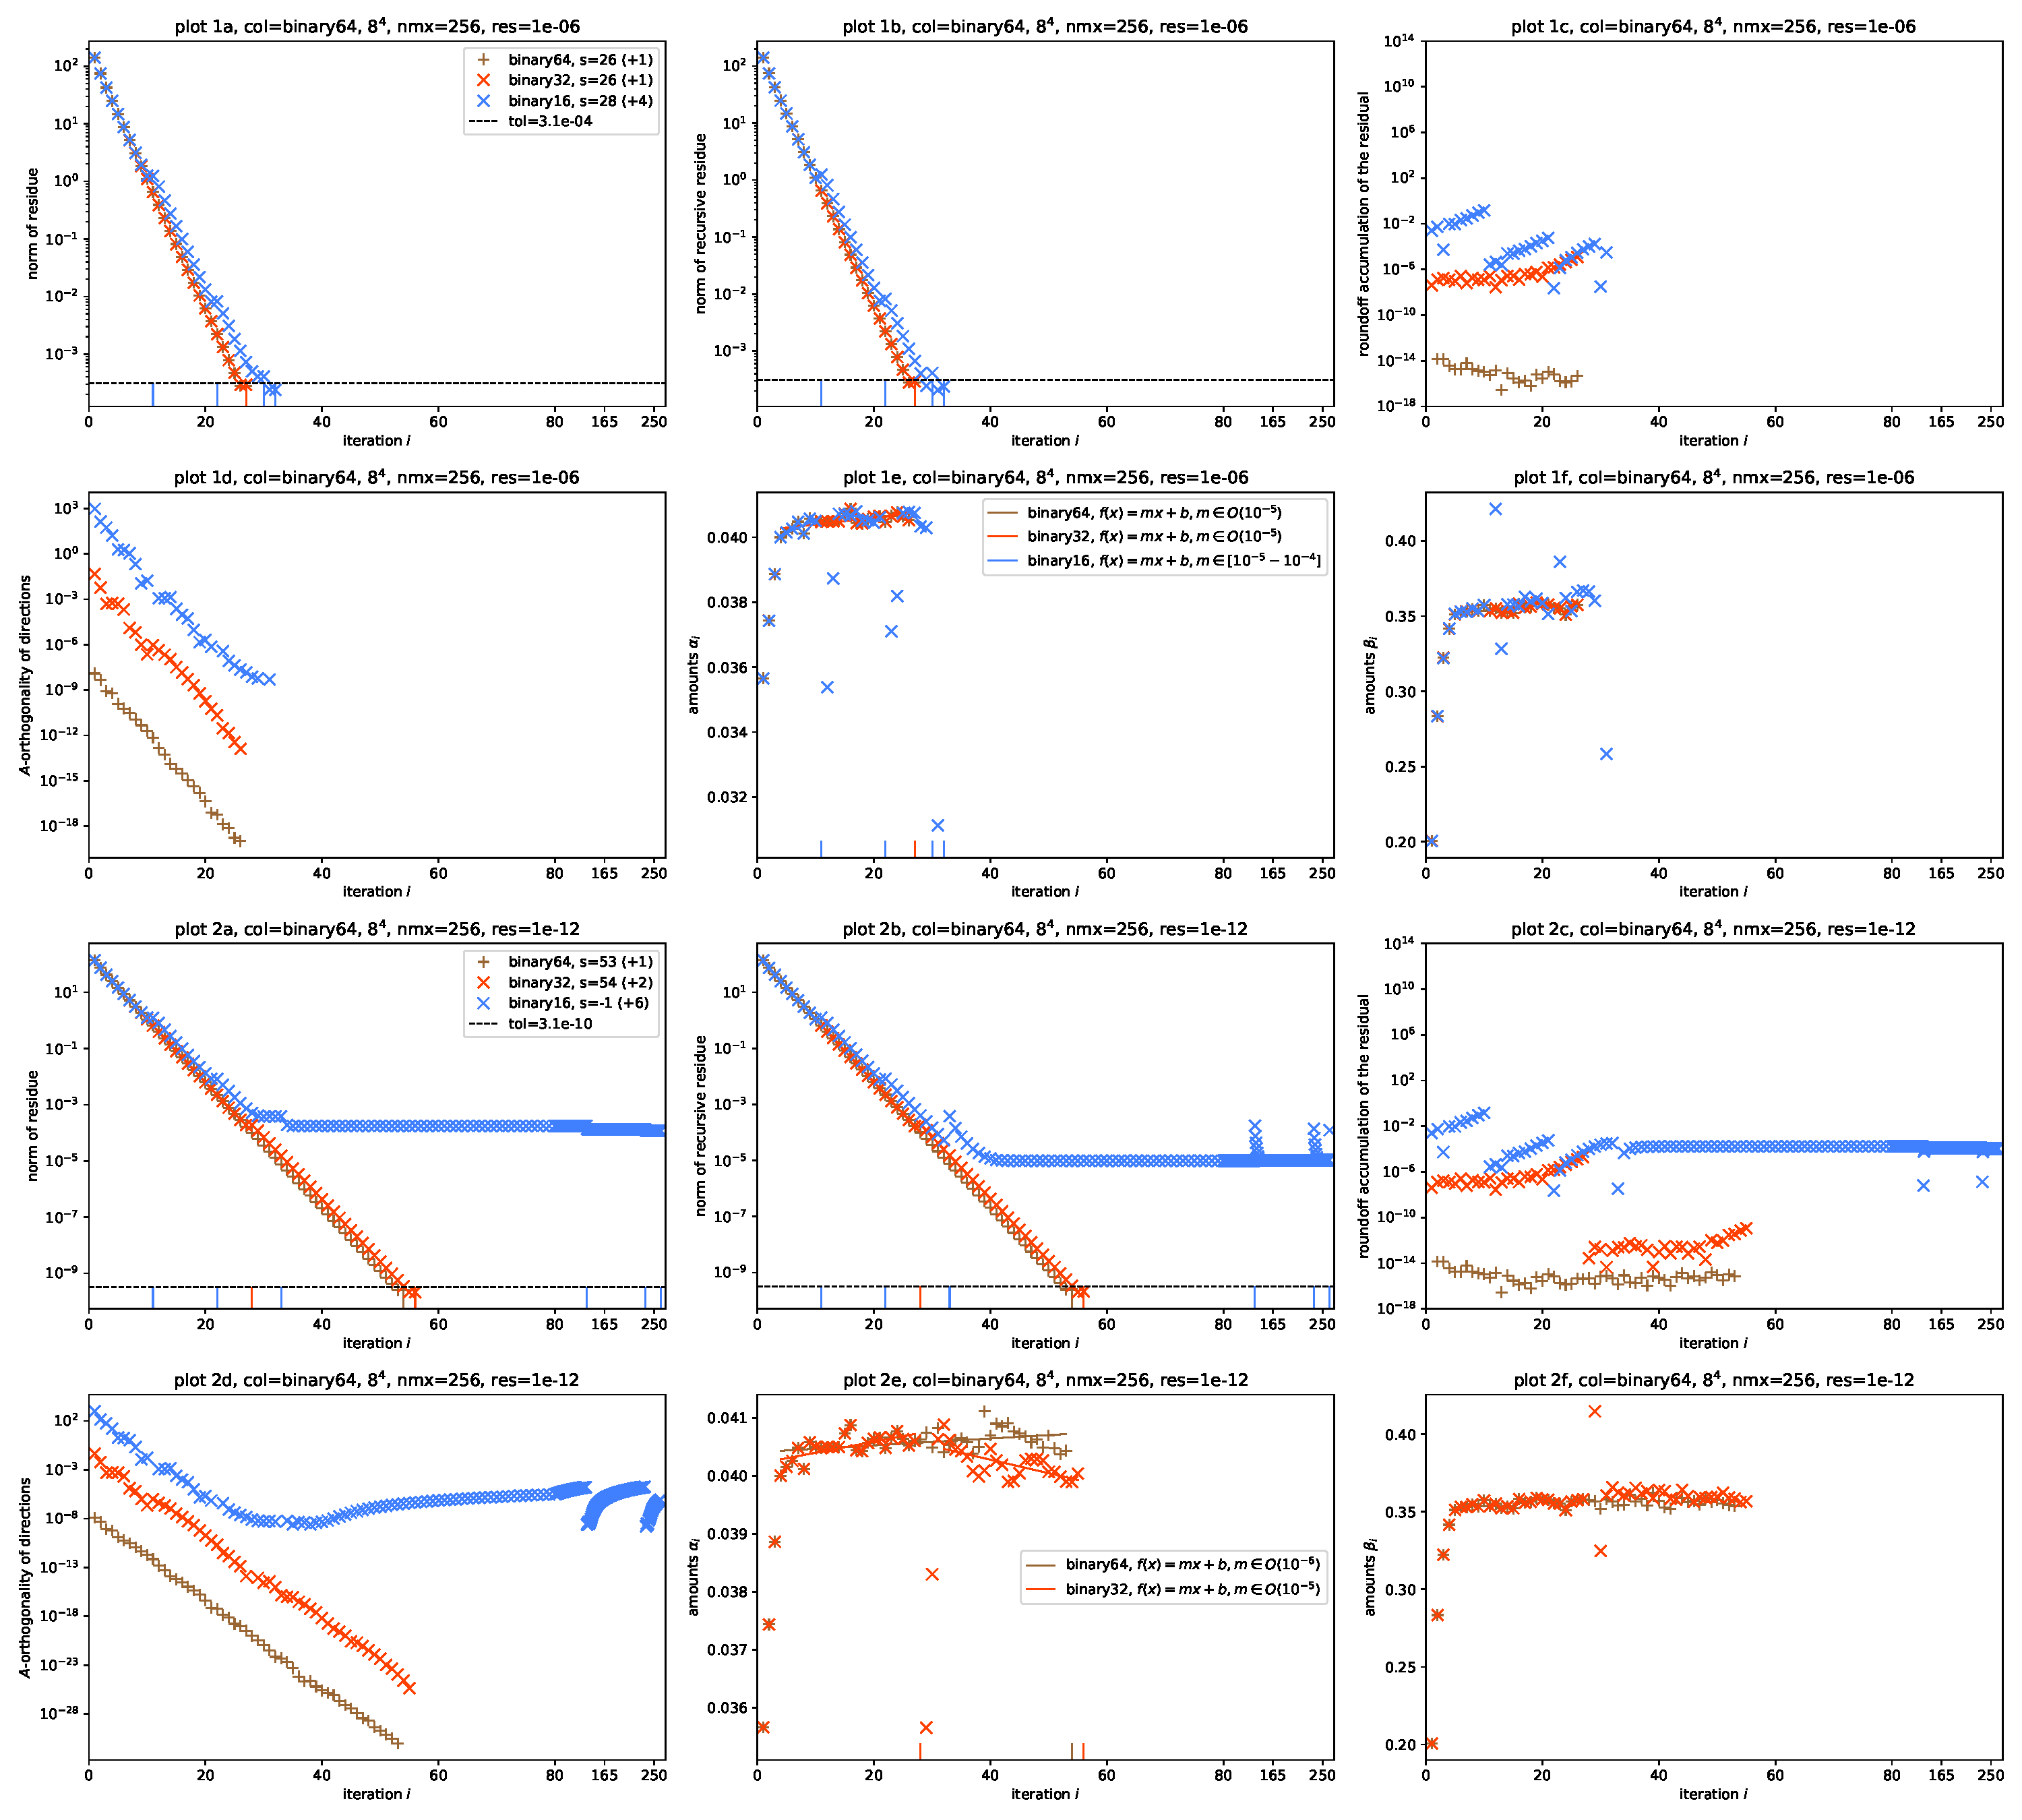
\includegraphics[width=1.0\textwidth]{plots/cgne_8x8x8x8_new}
    \caption{In anology to figures \ref{fig:cgne:col64} and \ref{fig:cgne:res12}. This time an $8^4$ lattice was used and only the floating point datatypes that are available in hardware nowadays were simulated. The \textit{first and second row} use \gls{binary64} as collective variable and $10^{-6}$ was the desired relative residual. The \textit{third and fourth row} have the exact same setup, but with a relative residual of $10^{-12}$ instead.}
    \label{fig:cgne8}
\end{figure}

\subsubsection{Conclusion}

The desicion between floats and posits is not trivial. It highly depends on how fast the machine can perform \acrshort{FLOPS} and \acrshort{POPS}. For example division in floating point arithmetic is very expensive (it may exceed \num{24} CPU cycles, many compiler optimizations evade them), whereas in posit arithmetic it is said to be cheap, because obtaining the inverse of a number is easy.

Another example could be that comparisons between floats are more expensive than for posits. Two posits are equal if their bit representations are equal. Comparing two floats is much more expensive, mainly because of the many \acrshortpl{nan} and since $0$ and $-0$ are equal but not bit-identical.

On the other hand, there is currently no hardware available, that has dedicated posit units and posits are not studied as intensive as floats. Floats are widespread, well understood and implemented in common hardware.

If one desides to replace \gls{binary32} with posits, the most elegant solution would be to naively replace the datatype and utilize \glspl{quire} in collective operations. To use \gls{binary64} collective variables is not recommended, because this would introduce many type conversions between the floating point and the posit format which is assumed to be expensive. The drawback ot this method is that \gls{posit16} may only converge if the relative residue is chosen high enough (see plot \textit{2a} in Figure \ref{fig:cgne:quire}).

If the desicion goes for floats, which might be the more realistic scenario, then the most elegant solution would be to use collective variables in \gls{binary64}. Type conversions between different IEEE floating point types are not considered to be expensive. The \gls{tensorfloat32} compared to \gls{binary32} and \gls{bfloat16} answers the question how important precision is in the calculation. All of them have the same number of exponent bits and therefore approximately the same number range, but very different precisions. We see that all of them were able to converge in any experiment, but with \gls{binary64} as collective variable, the results were closest to each other (see Figure \ref{fig:cgne:col64} plot \textit{3a}). The only real difference was in the amount of reset steps. If the datatype is lower in bitlength, the memory-boundedness suggests that the calculation performs faster, but the tradeoff is the amount of (computationally expensive) reset steps that increases with less precision. However, the datatype for collective operations should be precise and should have a large number range. Since the amount of variables needed in that datatype does not scale with the lattce size, it is perfectly right to use a datatype with large bitlength. Comparing the convergence of \gls{bfloat16} in the naive case (Figure \ref{fig:cgne:naive} plot \textit{1a}) with the case \gls{binary64} collective variables (Figure \ref{fig:cgne:col64} plot \textit{3a}), it can be seen that the algorithm converged \num{21} steps faster, only because the collective datatype was chosen to be \gls{binary64}. On the other hand, comparing the performance of \gls{binary16} in the two plots, we see that the number range of the collective datatype brought \gls{binary16} from no convergence to convergence within \code{status=35} steps - only marginally slower than \gls{binary32}. These arguments make \gls{binary64} the best choice for variables with a collective role.

\begin{proposal}[mixed precision]

TODO: proposal for mixed precision (binary16) conjugate gradient or other algorithms.

\end{proposal}

\begin{proposal}[approximating the amounts $\alpha_i$]

Looking at plot \textit{4e} of Figure \ref{fig:cgne:res12}, where the amounts $\alpha_i$ are plotted for every iteration, we see that after every reset step the amounts need $2-3$ step to reach a value that is not changing very much. This is becomes apparent when looking at the fitting lines. The values of the $\alpha_i$ are in the range $10^{-1}$ and the slopes $m$ of the fitting lines are in the range $10^{-4}$ - $10^{-5}$, suggesting that the value of $\alpha_i$ is not changing from iteration to iteration when only looking at $2-3$ significant decimal digits.

A possibility to reduce computational cost in each iteration could be to approximate the values of future $\alpha_i$ to be constant. The less precise the datatype, the larger the change in $\alpha_i$. The large error in $\alpha_i$ of \gls{bfloat16} suggests that the algorithm is not sensible to errors in $\alpha_i$. Therefore, it can be expected that the results should not change significantly with a approximated value of $\alpha_i$.

TODO:

\begin{itemize}
    \item adv1: residual can be calculated b-Ax, not recusively, no more roundoff accumulation, only roundoff errors
    \item adv2: only one matrix-vector multiplication per iteration, see dis2
    \item dis1: alpha approximation, can have errors
    \item dis2: the dirac operator must be given in form of Ddagger D as one operator
\end{itemize}

\end{proposal}

res $> 10^{-6}$

Simulated datatype: precision $>$ number range

Collective datatype: number range $>$ precision

res $< 10^{-6}$

Simulated datatype: precision $>$ number range

Collective datatype: number range $>$ precision

\section{SAP preconditioned GCR algorithm}

The next solver appearing in openQxD is called \code{SAP\_GCR}. It makes use of a multiplicative \acrfull{sap} as preconditioner for a flexible \acrfull{gcr} run.

TODO: motivation: parallel processing, chrial regime (spontaneous breaking of chiral symmetry), simulation containing sea-quarks limited to small lattices and large quark masses.

\subsection{Even-Odd Preconditioning}

Preconditioning in general, when employed in lattice QCD, is expected to have significant impact on the number of iterations of a solver. One way of preconditioning $D \psi = \eta$ is

\begin{align*}
    L D R \psi^{\prime} = L \eta,
\end{align*}

with $\psi = R^{-1} \psi^{\prime}$ and $L$, $R$ chosen wisely such that $LDR$ is well conditioned. If $L = \mathbb{I}$, it is called \df{right preconditioning}, if $R=\mathbb{I}$ it is called \df{left preconditioning}. If the Dirac-matrix involves only nearest-neighbor interactions it is possible to split the lattice into even and odd sites. If the sites are ordered such that the even sites come first,

\begin{align*}
    D &=
    \begin{pmatrix}
    D_{ee} & D_{eo} \\
    D_{oe} & D_{oo}
    \end{pmatrix},
    & & &
    \psi &=
    \begin{pmatrix}
    \psi_e \\
    \psi_o 
    \end{pmatrix}
\end{align*}

$D_{ee}$ and $D_{oo}$ consist of the interactions of even/odd sites among themselves, whereas $D_{eo}$ and $D_{oe}$ consider the interactions of even with odd sites. $\psi_e$ and $\psi_o$ contain the values for even and odd lattice sites of the spinor.

Using specific forms of $L$ and $R$, $D$ can be brought in a block-diagional form, namely

\begin{align*}
    L &= 
        \begin{pmatrix}
        1 & -D_{eo} D_{oo}^{-1} D_{oe} \\
        0 & 1
        \end{pmatrix}
    & &\text{and} &
    R &= 
        \begin{pmatrix}
        1 & 0 \\
        -D_{oo}^{-1} D_{oe} & 1
        \end{pmatrix}.
\end{align*}

After a bit of algebra,

\begin{align*}
    L D R &= 
        \begin{pmatrix}
        \hat{D} & 0 \\
        0 & D_{oo}
        \end{pmatrix},
    & &\text{with} &
    \hat{D} &= D_{ee} - D_{eo} D_{oo}^{-1} D_{oe}.
\end{align*}

This specific preconditioning reduces the amount of iterative steps needed by a factor of \num{2} approximately. The inversion of $D_{oo}$ is simple, because with only nearest-neighbor-interactions the odd sites do not interact among themselves, only with even sites. Thus $D_{oo}$ exhibits a diagonal form. Using

\begin{align*}
    D \psi = \eta \implies \begin{pmatrix}
    D_{ee} & D_{eo} \\
    D_{oe} & D_{oo}
    \end{pmatrix} \begin{pmatrix} \psi_e \\ \psi_o \end{pmatrix} = \begin{pmatrix} D_{ee} \psi_e + D_{eo} \psi_o \\ D_{oe}\psi_e + D_{oo} \psi_o \end{pmatrix} = \begin{pmatrix} \eta_e \\ \eta_o \end{pmatrix}
\end{align*}

we can write the preconditioned form, where only the even lattice sites have to be solved to determine $\psi_e$

\begin{align*}
    \hat{D} \psi_e &= D_{ee} \psi_e - D_{eo} D_{oo}^{-1} D_{oe} \psi_e \\
    &= ( \eta_e - D_{eo} \psi_o ) - D_{eo} D_{oo}^{-1} ( \eta_o - D_{oo} \psi_o ) \\
    &= \eta_e - D_{eo} D_{oo}^{-1} \eta_o,
\end{align*}

because $\psi_o$ follows from the solution $\psi_e$ via

\begin{align*}
    \psi_o = D_{oo}^{-1} (\eta_o - D_{oe} \psi_e).
\end{align*}


\subsection{Schwarz Alternating Procedure}

Domain decomposition is a way to partition the large system into (possibly many) smaller subproblems with regularly updated boundary conditions coming from solutions of neighboring subproblems. They fit very well into the notion of parallel processing, because each subproblem can be chosen to be contained in one single rank. The large lattice is split into sublattices called \df{local lattice}. Each rank has its own local lattice, the size of which is determined at compilation time. The full lattice consists of the ensemble of all local lattices. It is therefore adivable to chose the size of subproblems as a divisor of the local lattices such that at least one subproblem fits into one rank. These subproblems can then be solved using a \acrshort{gcr} solver.

The multiplicative \acrlong{sap} is such a domain decomposition method coming from the theory of partial differential equations. The domain decomposition preconditioner based on \acrshort{sap} involves itself an iterative procedure and is therefore very expensive.


\subsection{Generalized Conjugate Residual algorithm}

We wish to solve \eqref{eq:Axb} if a is not Hermitian. Comparing to the conjugate gradient algorithm, we minimize the residual $\vec{r}$ of the solution $\vec{x}$, using the \df{quadratic form},

\begin{align*}
    f(\vec{x}) &= \frac{1}{2} \left( \vec{b} - A \vec{x} \right)^{\dagger} \left( \vec{b} - A \vec{x} \right) + c \\
               &= \frac{1}{2} \norm{ \vec{b} - A \vec{x} }^2 + c\\
               &= \frac{1}{2} \norm{ \vec{r} }^2 + c.
\end{align*}

where $c \in \mathbb{C}$. When taking the derivative of this function with repect to $\vec{x}$, we find that

\begin{align*}
    f'(\vec{x}) = A^{\dagger} A \vec{x} - A^{\dagger} \vec{b}.
\end{align*}

\begin{lemma}[Uniqueness of the solution]
The solution $\vec{x}$ in equation \eqref{eq:Axb} is unique and the global minimum of $f(\vec{x})$, if $A$ is non-singular.
\end{lemma}

\begin{proof}
Let us rewrite $f(\vec{p})$ at an arbitrary point $\vec{p} \in \mathbb{C}$ in terms of the solution vector $\vec{x}$,

\begin{align*}
    f(\vec{p}) &= \frac{1}{2} \left( \vec{b} - A \vec{p} \right)^{\dagger} \left( \vec{b} - A \vec{p} \right) + c + f(\vec{x}) - f(\vec{x}) \\
    &= f(\vec{x}) + \frac{1}{2} \vec{p}^{\dagger} (A^{\dagger} A) \vec{p} - \frac{1}{2} (A \vec{p})^{\dagger} \vec{b} - \frac{1}{2} \vec{b}^{\dagger} (A \vec{p}) + \frac{1}{2} \vec{b}^{\dagger} \vec{b} \\
    &= f(\vec{x}) + \frac{1}{2} (\vec{p} - \vec{x})^{\dagger} (A^{\dagger} A) (\vec{p} - \vec{x}) + \frac{1}{2} (A \vec{p})^{\dagger} (\textcolor{cyellow}{A \vec{x}}) + \frac{1}{2} (\textcolor{cyellow}{A \vec{x}})^{\dagger} (A \vec{p}) - \frac{1}{2} (\textcolor{cyellow}{A \vec{x}})^{\dagger} (\textcolor{cyellow}{A \vec{x}}) \\
    &\phantom{==} - \frac{1}{2} (A \vec{p})^{\dagger} \textcolor{cyellow}{\vec{b}} - \frac{1}{2} \textcolor{cyellow}{\vec{b}}^{\dagger} (A \vec{p}) + \frac{1}{2} \textcolor{cyellow}{\vec{b}}^{\dagger} \textcolor{cyellow}{\vec{b}} \\
    &= f(\vec{x}) + \frac{1}{2} (\vec{p} - \vec{x})^{\dagger} (A^{\dagger} A) (\vec{p} - \vec{x}) \\
\end{align*}

where to obtain the last line, $\textcolor{cyellow}{A \vec{x}} = \textcolor{cyellow}{\vec{b}}$ as used, thus the term simplified.

In the new form of $f(\vec{p})$, one can directly see that, $\vec{x}$ must minimize the function:

\begin{align*}
    f(\vec{p}) &= f(\vec{x}) + \frac{1}{2} (\vec{p} - \vec{x})^{\dagger} (A^{\dagger} A) (\vec{p} - \vec{x}) \numberthis \label{eq:fp_gcr} \\
    &= f(\vec{x}) + \frac{1}{2} \underbrace{ \norm{ A (\vec{p} - \vec{x})}^2 }_{\text{$> 0$ for $\vec{p} \neq \vec{x}$}}.
\end{align*}

Therefore $\vec{x}$ is the global unique minimum if $A$ is non-singular.

\end{proof}

\begin{remark}
Notice the similarity of the above equation \eqref{eq:fp_gcr} to the analogue of the conjugate gradient algorithm \eqref{eq:fp_cgne}. The only difference is the substitution of $A \longmapsto A^{\dagger} A$. It is therefore advisable in the derivation of an algorithm to require the directions $\vec{p}_i$ to be $A^{\dagger} A$-orthogonal instead of $A$-orthogonal.
\end{remark}

In the same manner as in the derivation of the method of conjugate gradient, we impose a iterative \df{step equation} to be

\begin{align*}
    \vec{x}_{i+1} = \vec{x}_i + \alpha_i \vec{p}_i,
\end{align*}

again with \df{directions} $\vec{p}_i$ and \df{amounts} $\alpha_i$ that have to be determined. The recursively calculated \df{residual} has again the same formula

\begin{align*}
    \vec{r}_{i+1} = \vec{r}_i - \alpha_i A \vec{p}_i.
\end{align*}

Imposing $A^{\dagger} A$-orthogonality instead of regular $A$-orthogonality between error $\vec{e}_{i+1}$ and direction $\vec{p}_i$,

\begin{align*}
    0 &\stackrel{!}{=} \vec{e}_{i+1}^{\dagger} (A^{\dagger} A) \vec{p}_i \\
                    &= ( \vec{e}_{i} + \alpha_i \vec{p}_i )^{\dagger} A^{\dagger} A \vec{p}_i \\
\end{align*}

gives us an expression for the amounts $\alpha_i$. Notice the above equation is equivalent to imposing $A$-orthogonality $0=\vec{r}_{i+1}^{\dagger} A \vec{p}_i$. However, we find (compare equation \eqref{eq:cgne:alpha_pre})

\begin{align*}
      \alpha_i = \frac{ \vec{r}_i^{\dagger} (A \vec{p}_{i}) }{ \vec{p}_i^{\dagger} (A^{\dagger} A) \vec{p}_i } = \frac{ \vec{r}_i^{\dagger} (A \vec{p}_{i}) }{ \norm{A \vec{p}_i}^2 }.
\end{align*}

The \acrshort{gcr} algorithm does store all previous direction $\vec{p}_i$ as well as $A \vec{p}_i$ in contrast to conjugate gradient. Thus the derivation changes slightly. Let's continue with the determination of the directions using \df{Gram-Schmidt orthogonalisation} by imposing $A^{\dagger} A$-orthogonality instead of $A$-orthogonality and without imposing all previous $\beta_{ij}$ to be zero (see definition \ref{df:gramschmidt}). Likewise, we set $\vec{u}_i = \vec{r}_i$ and find

\begin{align*}
    \begin{split}
        \vec{p}_0 &= \vec{r}_0 \\
        \vec{p}_{i+1} &= \vec{r}_{i+1} + \sum_{j=0}^{i} \beta_{ij} \vec{p}_j,
    \end{split}
\end{align*}

with

\begin{align*}
    \beta{ij} = - \frac{ \vec{r}_{i+1}^{\dagger} A^{\dagger} A \vec{p}_j }{ \vec{p}_j^{\dagger} A^{\dagger} A \vec{p}_j } = - \frac{ (A \vec{r}_{i+1})^{\dagger} (A \vec{p}_j) }{ \norm{A \vec{p}_j}^2 }.
\end{align*}

Using the above equations, we find the final form of the \df{Generalized Conjugate Residuals Method}.

\begin{definition}[Generalized Conjugate Residuals Method]

\label{df:gcr}

The iteration step equation of the \df{Generalized Conjugate Residuals Method} in defined as

\begin{align}
    \vec{x}_{i+1} = \vec{x}_i + \alpha_i \vec{p}_i, \label{eq:gcr:step}
\end{align}

with

\noindent\begin{minipage}{.5\linewidth}
    \begin{align*}
        \vec{r}_{i+1} &= \vec{r}_{i}   - \alpha_i A  \vec{p}_i, \\
        \vec{p}_{i+1} &= \vec{r}_{i+1} + \sum_{j=0}^{i} \beta_{ij} \vec{p}_j, 
    \end{align*}
\end{minipage}
\begin{minipage}{.5\linewidth}
    \begin{align}
        \alpha_i  &=   \frac{ \vec{r}_i^{\dagger} (A \vec{p}_{i}) }{ \norm{A \vec{p}_i}^2 }, \label{eq:gcr:alpha} \\
        \beta{ij} &= - \frac{ (A \vec{r}_{i+1})^{\dagger} (A \vec{p}_j) }{ \norm{A \vec{p}_j}^2 },
    \end{align}
\end{minipage}

and initial starting vectors

\begin{align*}
    \vec{x}_{0} &= \text{arbitrary starting point}, \\
    \vec{p}_{0} &= \vec{r}_{0} = \vec{b} - A \vec{x}_0.
\end{align*}

\end{definition}

There are some remarks to note about the method of \acrshort{gcr}.

\begin{remark}
    After calculating $\vec{r}_{i+1}$ and $A \vec{r}_{i+1}$, we can recursively determine $A \vec{p}_{i+1}$ via 

    \begin{align}
        A \vec{p}_{i+1} &= A \vec{r}_{i+1} + \sum_{j=0}^{i} \beta_{ij} A \vec{p}_j. \label{eq:gcr:Api}
    \end{align}

    This limits the number of matrix-vector products to one per iteration.

\end{remark}

\begin{remark}
    All previous $\vec{p}_i$ and $A\vec{p}_i$ need to be stored in memory in order to construct the next $\vec{p}_{i+1}$ and $A \vec{p}_{i+1}$.
\end{remark}

\begin{remark}
    Comparing to the conjugate gradient algorithm, we imposed $A^{\dagger} A$-orthogonality of the directions $\vec{p}_i$ instead of $A$-orthogonality as well as $A$-orthogonality of $\vec{r}_{i+1}$ and $\vec{p}_i$ instead of regular orthogonality. A vanishing of all previous $\beta_{ij}$ on the other hand was not imposed, leading to the sum in the recursive relation of $\vec{p}_{i+1}$.
\end{remark}

\subsection{GCR in openQxD}

The actual implementation of the \acrshort{gcr} algorithm in openQxD is quite different\footnotemark, but actually equivalent to the definition \ref{df:gcr}. Ref. \cite{luscher2004} explains the implementation of the algorithm in detail. The main \acrshort{gcr}-loop looks as in Algorithm \ref{alg:gcr} (see Figure 3 in \cite{luscher2004})

\footnotetext{See \code{fgcr()} in \code{modules/linsolv/fgcr.c} lines \num{212}ff in \cite{openqxd}.}

\begin{figure}
\centering
\begin{minipage}{.6\linewidth}
\begin{algorithm}[H]
\SetAlgoLined
  $\rho_0 = \eta$ \;
  \For{$k \gets 0, 1, 2$ \KwTo $n_{kv}$}{
    $\phi_k = M_{sap} \rho_k$ \;
    $\chi_k = D \phi_k$ \;
    \For{$l \gets 0$ \KwTo $k - 1$}{
      $a_{lk} = (\chi_l, \chi_k)$ \;
      $\chi_k = \chi_k - a_{lk} \chi_l$ \;
    }
    $b_k = \norm{\chi_k}$ \;
    $\chi_k = \frac{\chi_k}{b_k}$ \;
    $c_k = (\chi_k, \rho_k)$ \;
    $\rho_{k+1} = \rho_k - c_k \chi_k$ \;
 }
 \caption{Pseudo-code for the GCR recursion.}
 \label{alg:gcr}
\end{algorithm}
\end{minipage}
\end{figure}

In the algorithm above, $M_{sap}$ is the \acrlong{sap} preconditioner, that might depend on the iteration number $k$ as well, making the algorithm flexible. $D$ is the Dirac-operator and $\rho_k$ the residual in the $k$-th step. The algorithm does not include a update of the solution vector $\psi_{k+1}$, instead this is done after $n_{kv}$ iterations all at once,

\begin{align}
    \psi_{k+1} = \sum_{l=0}^k \alpha^{\prime}_l \rho_k. \label{eq:gcr:step:paper}
\end{align}

\begin{lemma}
The iterative algorithm from definition \ref{df:gcr} is equivalent to algorithm \ref{alg:gcr} when setting the preconditioning operator $M_{sap} = \mathbb{I}$, the Dirac-matrix $D = A$, the source vector $\eta = \vec{b}$ and the solution vectors $\psi_k = \vec{x}_k$.
\end{lemma}

\begin{proof}

Noticing that the residual $\rho_k = \vec{r}_k$ from line \num{12} in algorithm \ref{alg:gcr} and in definition \ref{df:gcr} must be identical, we find that $\chi_k$ must be proportional to $A \vec{p}_k$. Before the normalization in line \num{10}, we have $\chi_k = A \vec{p}_k$. The $b_k = \norm{\chi_k}$ are set before normalisation of $\chi_k$, therefore $b_k = \norm{\chi_k} = \norm{A \vec{p}_k}$. Using this we find $a_{lk} = (\chi_l, D \rho_k)$ and since $l < k$ the $\chi_l$ are normalied, thus $\chi_l = b_l A \vec{p}_l$ after line \num{10}. Thus $a_{lk} = (A \vec{p}_l, D \rho_k)/b_l = - \beta_{k-1,l} \norm{A \vec{p}_l}$. Finally, the $c_k$ are defined after normalization of the $\chi_k$, therefore they evaluate to $c_k = (\chi_k, \rho_k) = (A \vec{p}_k, \vec{r}_k)/b_k = \alpha_k \norm{A \vec{p}_k}$. Using these substitutions we find the same formulas as in definition \ref{df:gcr}, except for the step equation.

The main difference between the step equations \eqref{eq:gcr:step} and \eqref{eq:gcr:step:paper} is that in the former the solution $\vec{x}_{i+1}$ is spanned by the direction vectors $\vec{p}_i$, whereas in the latter it is spanned by the residuals $\rho_i = \vec{r}_i$. This is not a problem since both sets of vectors span the same space, but the amounts $\alpha^{\prime}_l$ in equation \eqref{eq:gcr:step:paper} differ heavily from the amounts $\alpha_i$ in equation \eqref{eq:gcr:alpha}.

To determine the amounts $\alpha^{\prime}_l$ in terms of $\alpha_i$ and $\beta_{ij}$, we notice equation \eqref{eq:gcr:Api},

\begin{align}
    A \vec{p}_{i} = A \vec{r}_{i} + \sum_{j=0}^{i-1} \beta_{i-1,j} A \vec{p}_j &\iff b_{i} \chi_{i} = D \rho_i - \sum_{j=0}^{i-1} a_{ji} \chi_j \label{eq:gcr:Api:equiv}
\end{align}

and the fact that

\begin{align}
    \rho_{k+1} = \eta - \sum_{l=0}^k c_l \chi_l. \label{eq:gcr:paper:rho1}
\end{align}

But also 

\begin{align*}
    \rho_{k+1} &= \eta - D \psi_{k+1} \\
    &= \eta - \sum_{l=0}^k \alpha^{\prime}_l D \rho_k \\
    &= \eta - \sum_{l=0}^k \alpha^{\prime}_l \left[ b_k \chi_k + \sum_{j=0}^{k-1} a_{jk} \chi_j \right], \numberthis \label{eq:gcr:paper:rho2}
\end{align*}    

where in the last step equation \eqref{eq:gcr:Api:equiv} was inserted. The $\chi_i \propto A \vec{p}_i$ are linearly independent, thus the coefficients from \eqref{eq:gcr:paper:rho2} can be compared to \eqref{eq:gcr:paper:rho1}, giving for $m=0, 1, \dots, k$

\begin{align*}
    \alpha^{\prime}_m &= \frac{1}{b_m} \left[ c_m + \sum_{l=m+1}^k \alpha^{\prime}_l a_{ml} \right] \\
    &= \alpha_m - \sum_{l=m+1}^k \alpha^{\prime}_l \beta_{l-1,m}.
\end{align*} 

\end{proof}

\section{Deflated SAP preconditioned GCR algorithm}

TODO

\section{Summary}

TODO

\newpage

\bibliography{include/references}
\bibliographystyle{abbrv}

\newpage

\appendix
\section*{Appendices}
\addcontentsline{toc}{section}{Appendices}
\renewcommand{\thesubsection}{\Alph{subsection}}

\subsection{Code}
\label{sec:code}

All code used in this report is open source and can be found in the GitHub repository \cite{github}

\printglossary[type=\acronymtype]

\printglossary

\end{document}

